\documentclass[11pt,aspectratio=169]{beamer}

\usepackage[T1,T2A]{fontenc}
\usepackage[utf8]{inputenc}
\usepackage[russian]{babel}
\usepackage{anyfontsize}

\usepackage{graphicx}

\usetheme{Boadilla}
\selectcolormodel{gray}

% \setbeamertemplate{footline}[page number]
\setbeamertemplate{footline}{\hfill\insertframenumber/\inserttotalframenumber\hspace*{2mm}\vspace*{1mm}}
% \setbeamertemplate{footline}{}

% \usecolortheme{rose}

\usefonttheme{professionalfonts}
% \usefonttheme{serif}
\useinnertheme{circles}

\beamertemplatenavigationsymbolsempty

\vspace*{15pt}
\title{Модель заполняемости \\ и ценообразования РЖД}
\author{}
\institute{}
\date{}

\begin{document}

\maketitle

\begin{frame}
    \frametitle{Доля заполненных данных за 30-дневный период}

    \begin{figure}
        \centering
        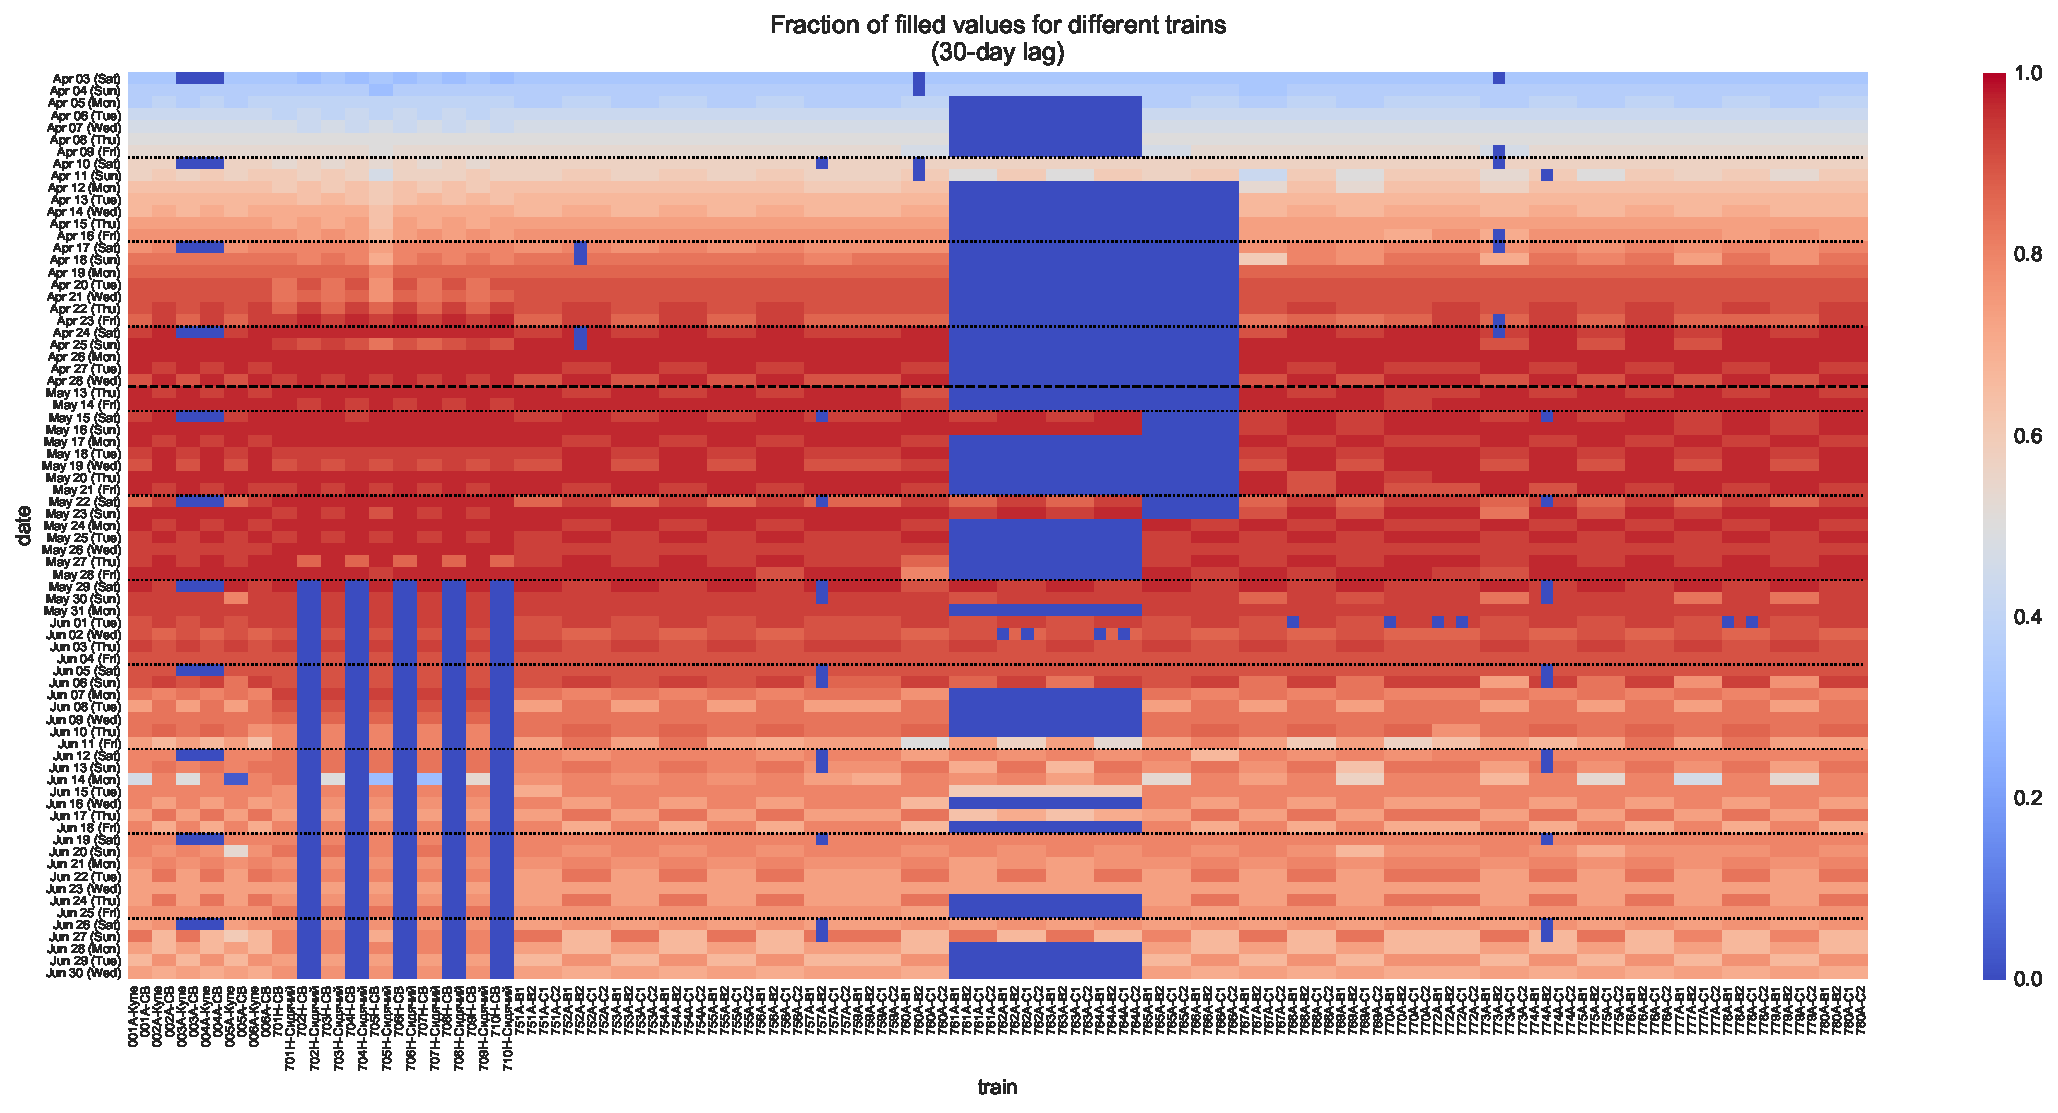
\includegraphics[width=\textwidth]{../data/figures/filled_frac.pdf}
    \end{figure}

\end{frame}


\begin{frame}
    \frametitle{Доля заполненных данных за 30-дневный период (очищ.)}

    \begin{figure}
        \centering
        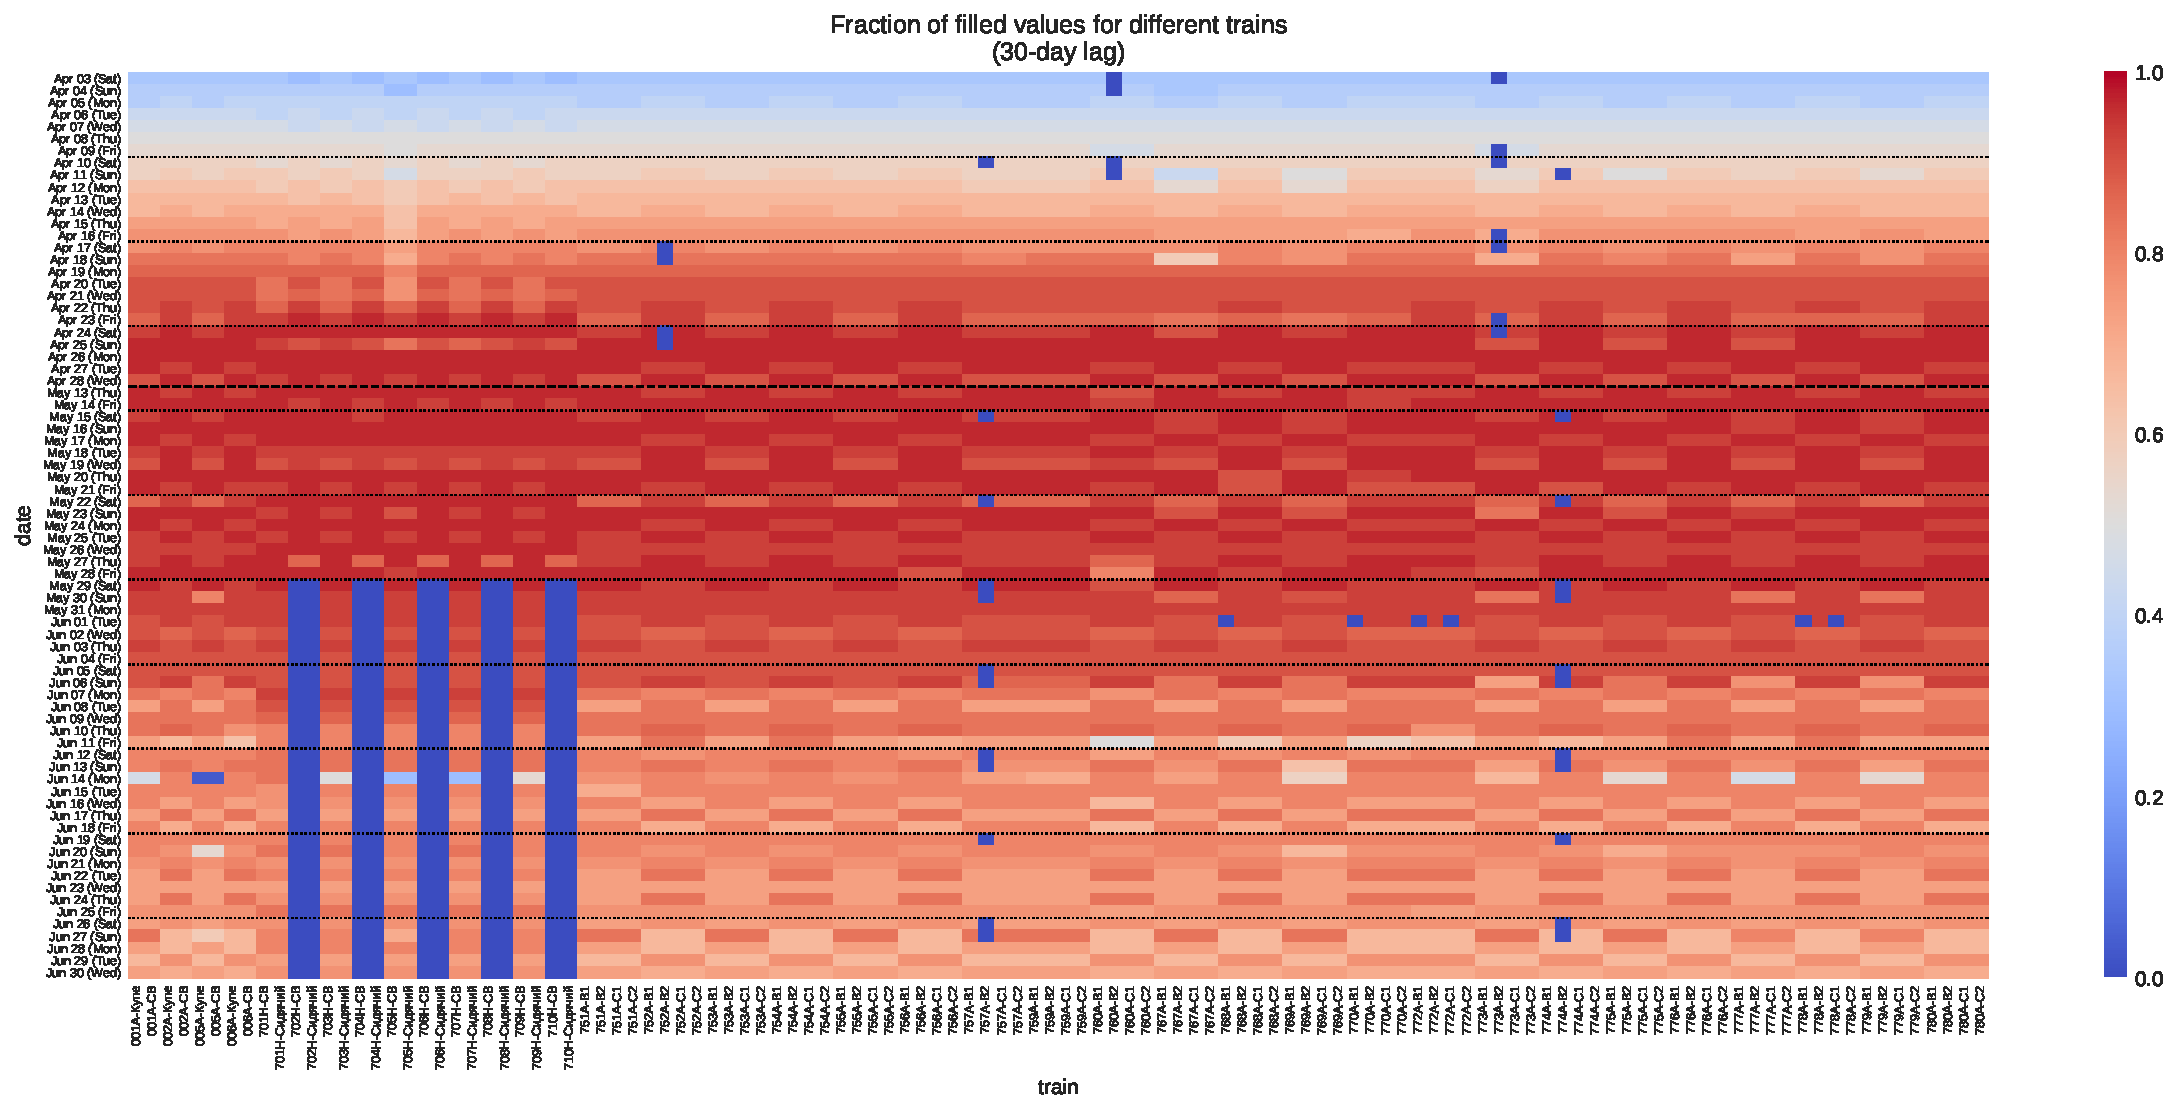
\includegraphics[width=\textwidth]{../data/figures/filled_frac_clean.pdf}
    \end{figure}

\end{frame}

\begin{frame}
    \frametitle{Доля вместимости относительно общей}

    \begin{figure}
        \centering
        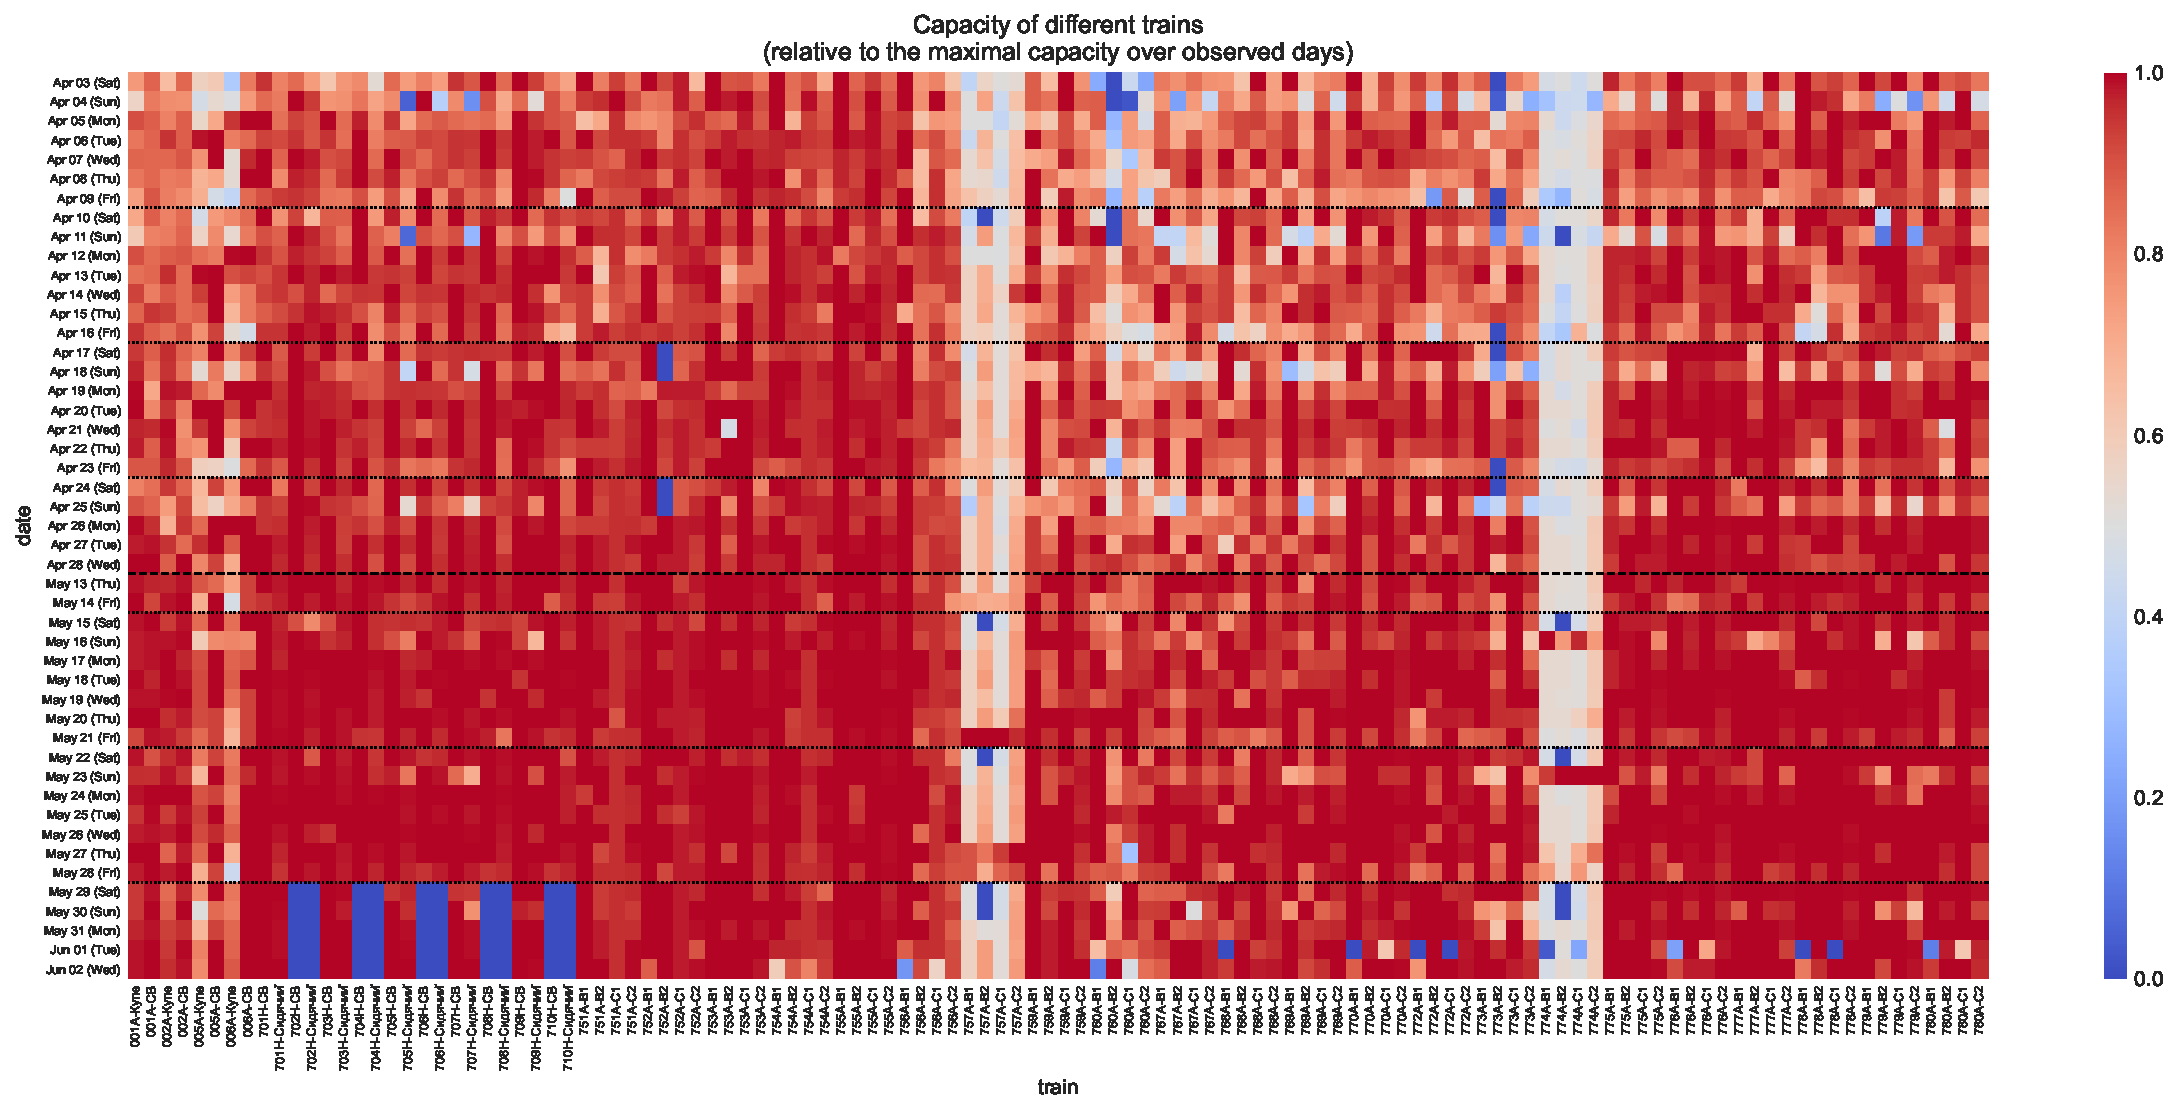
\includegraphics[width=\textwidth]{../data/figures/capacity.pdf}
    \end{figure}

\end{frame}


\begin{frame}
    \frametitle{Доля вместимости относительно общей (очищ.)}

    \begin{figure}
        \centering
        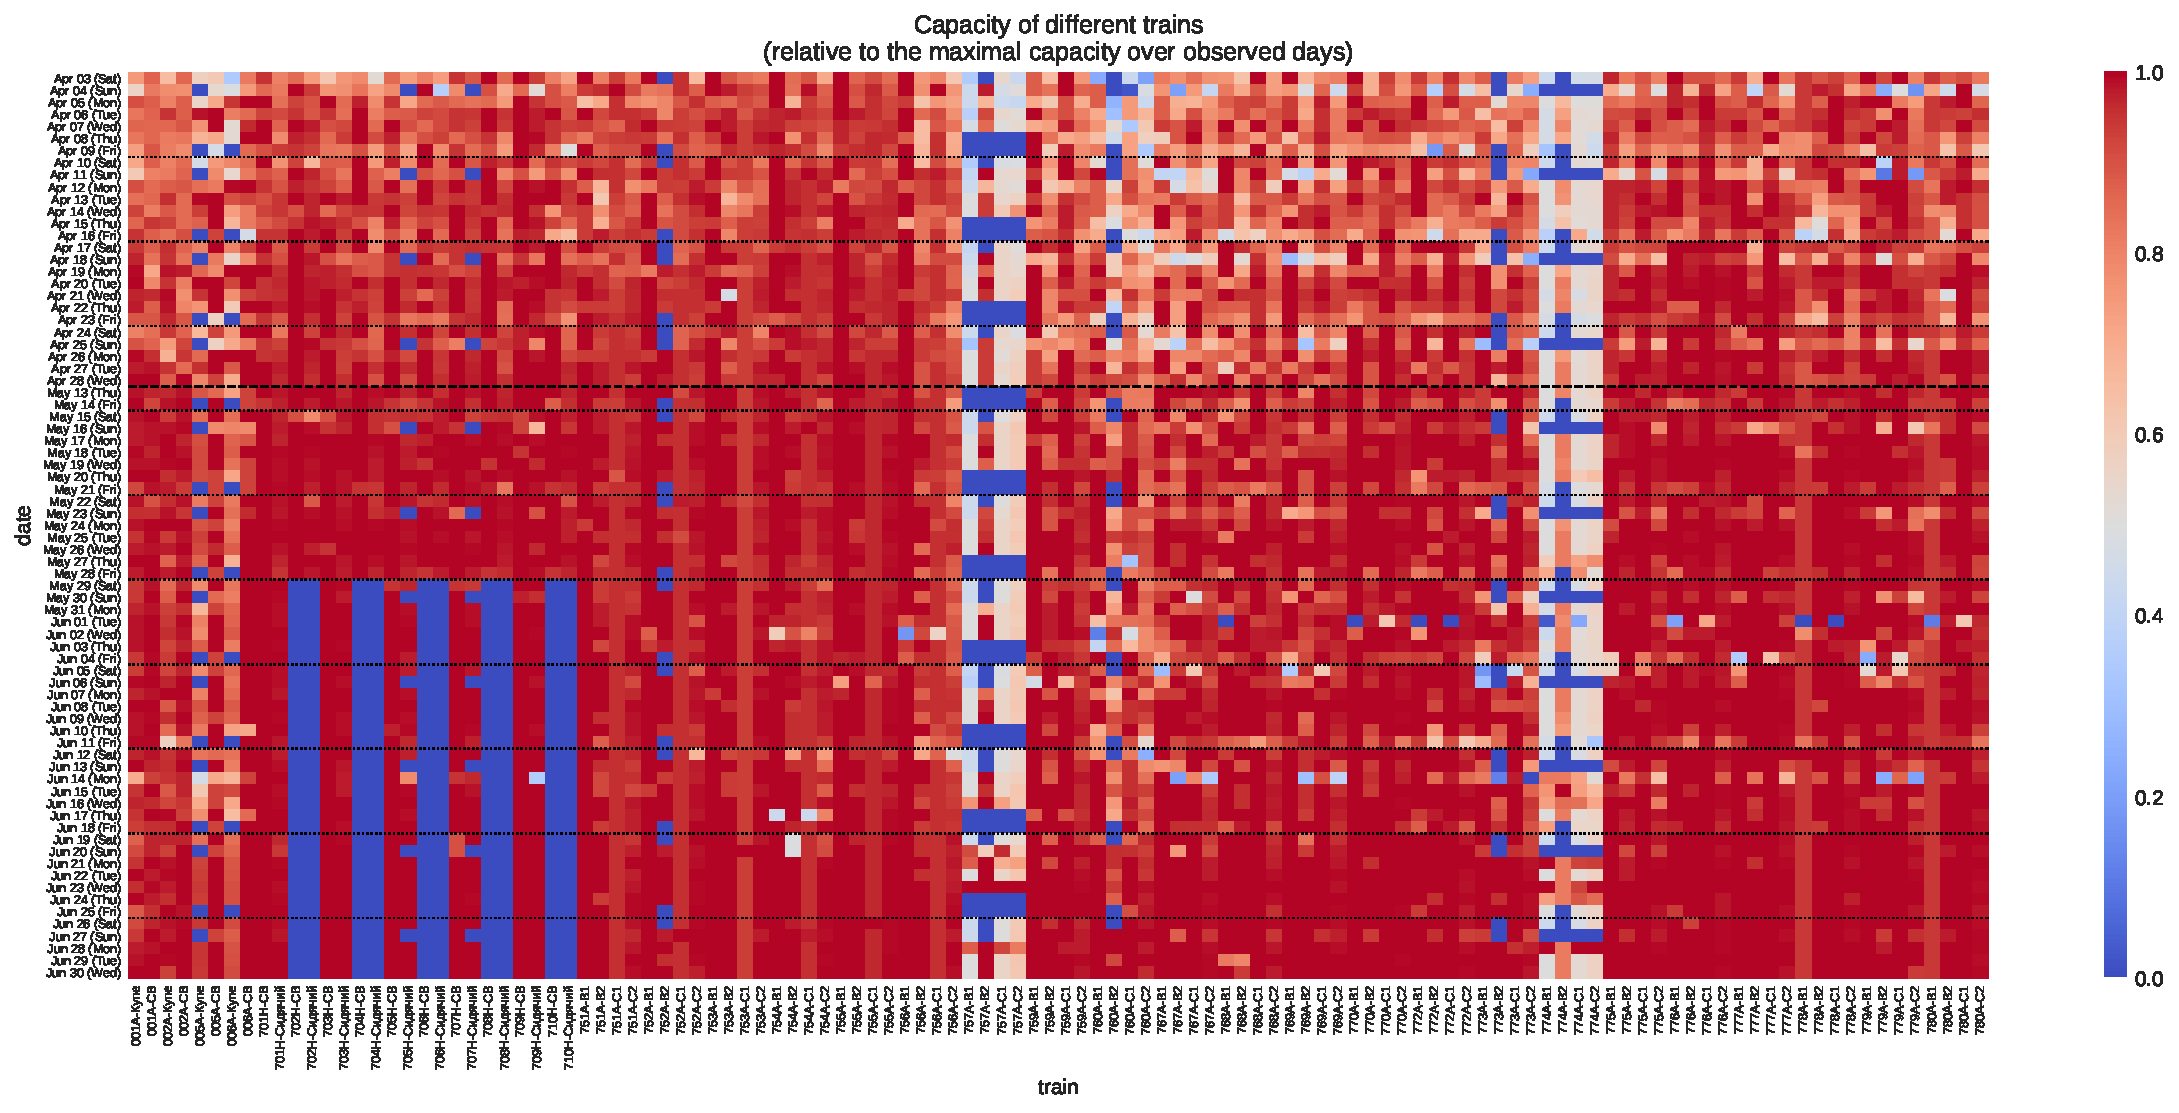
\includegraphics[width=\textwidth]{../data/figures/capacity_clean.pdf}
    \end{figure}

\end{frame}


\begin{frame}
    \frametitle{Свободные места по дням недели}

    \begin{figure}
        \centering
        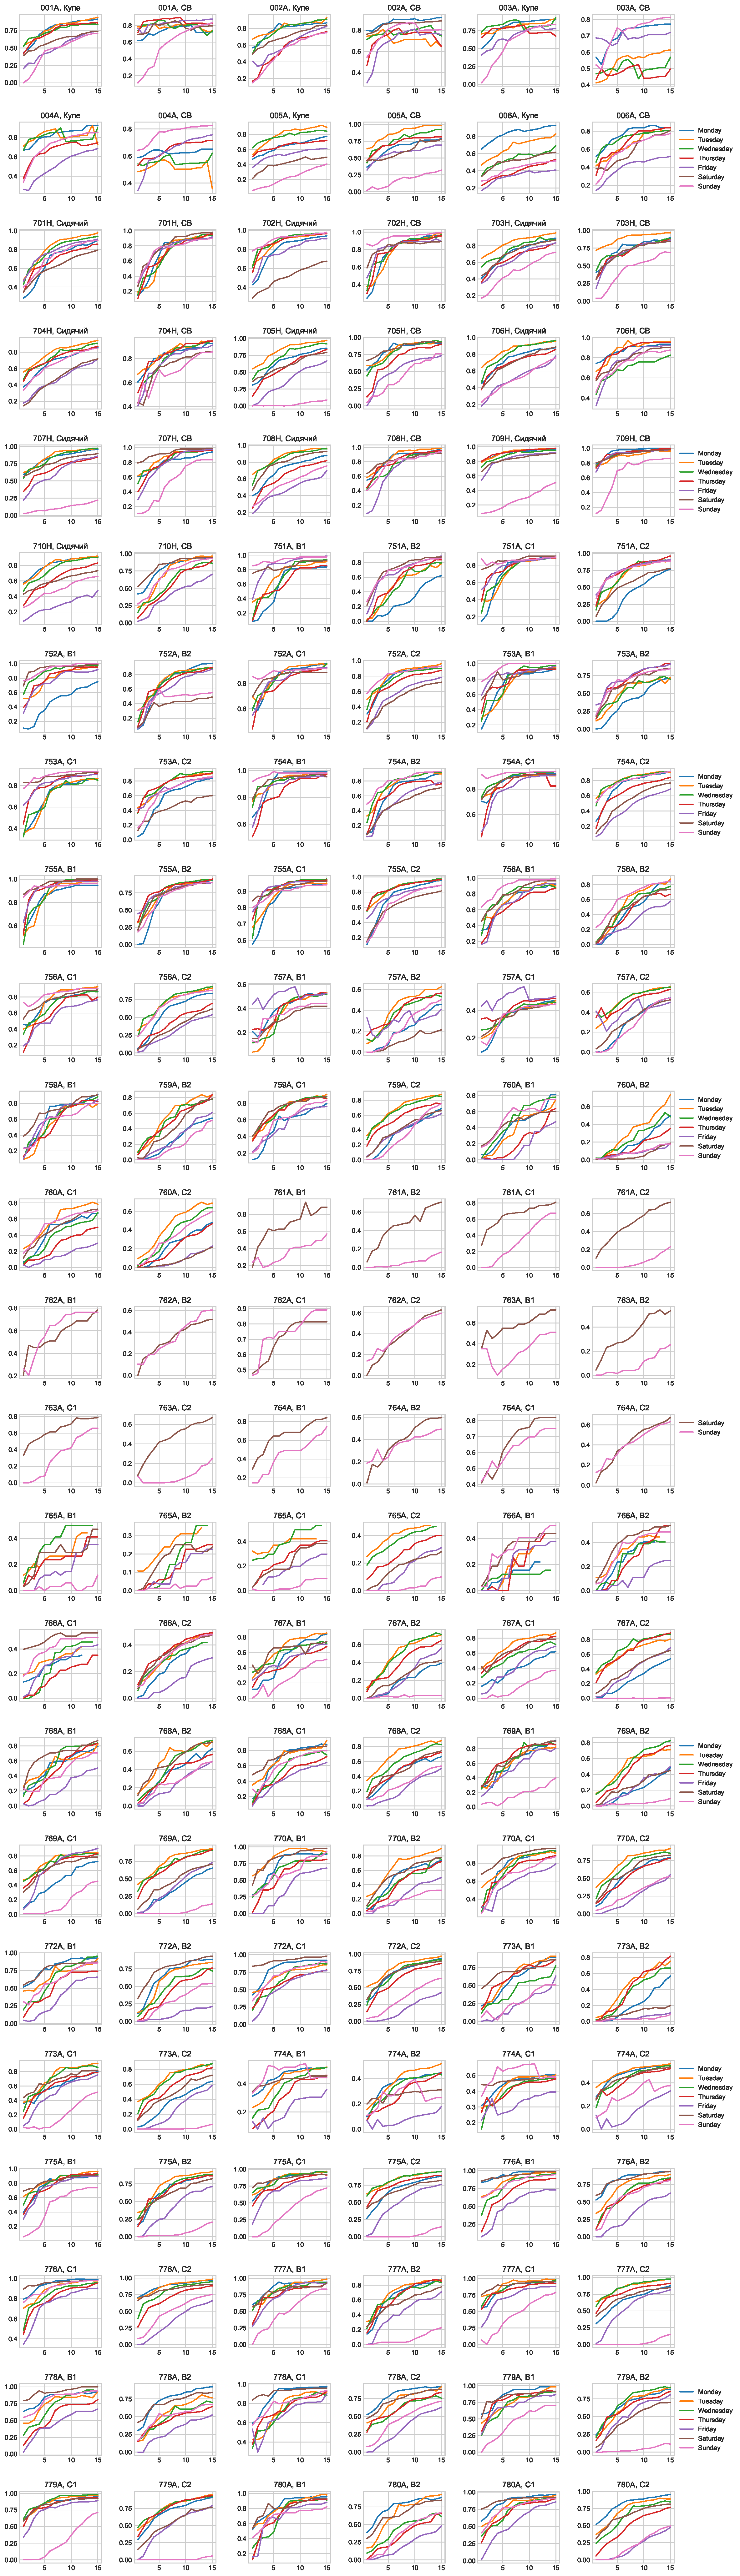
\includegraphics[width=\textwidth]{../data/figures/places_vs_weekday.pdf}
    \end{figure}

\end{frame}



\begin{frame}
    \frametitle{Значения метрик моделей}

    \begin{figure}
        \centering
        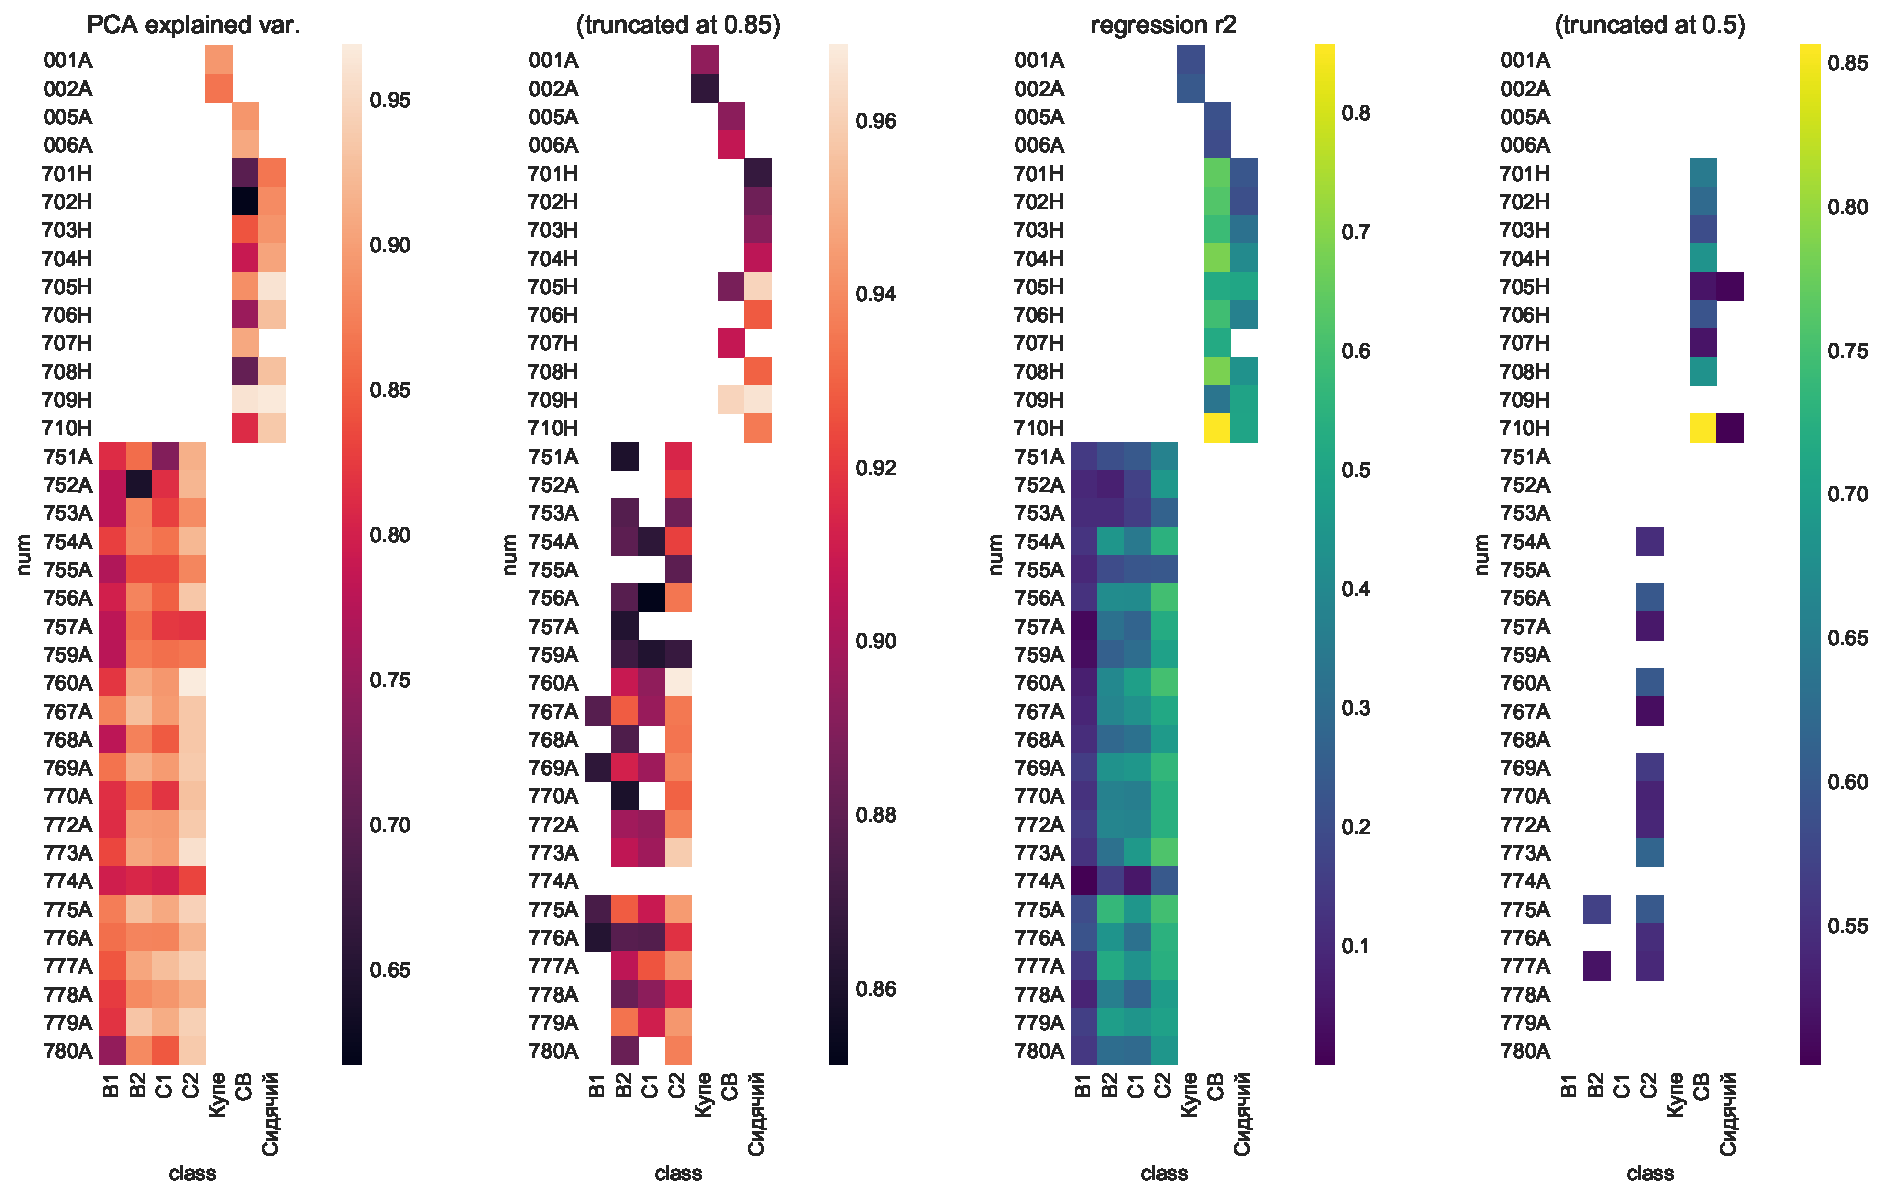
\includegraphics[height=0.92\textheight]{../data/figures/model_metrics.pdf}
    \end{figure}

\end{frame}


\begin{frame}
    \frametitle{Объясняем объяснённую дисперсию}

    \begin{figure}
        \centering
        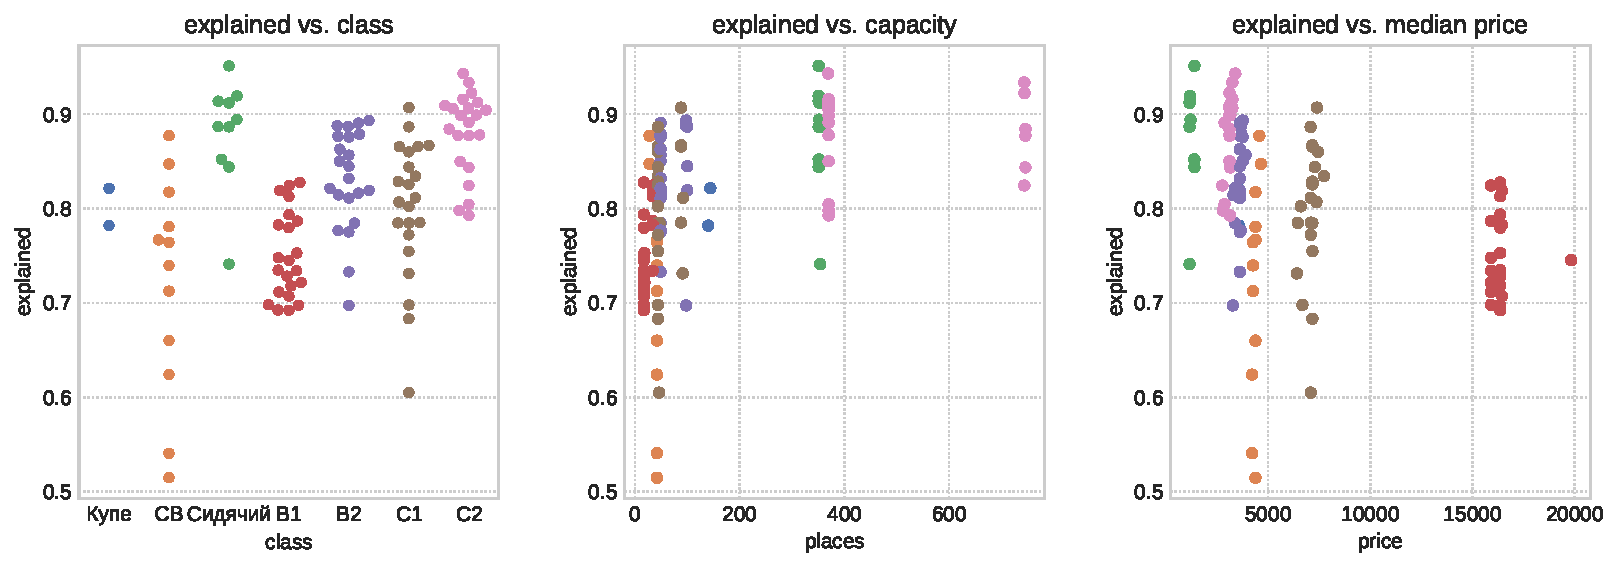
\includegraphics[width=\textwidth]{../data/figures/explaining_explained_variance.pdf}
    \end{figure}

\end{frame}


\begin{frame}
    \frametitle{Поезда с низкой объяснённой дисперсией}

    \begin{figure}
        \centering
        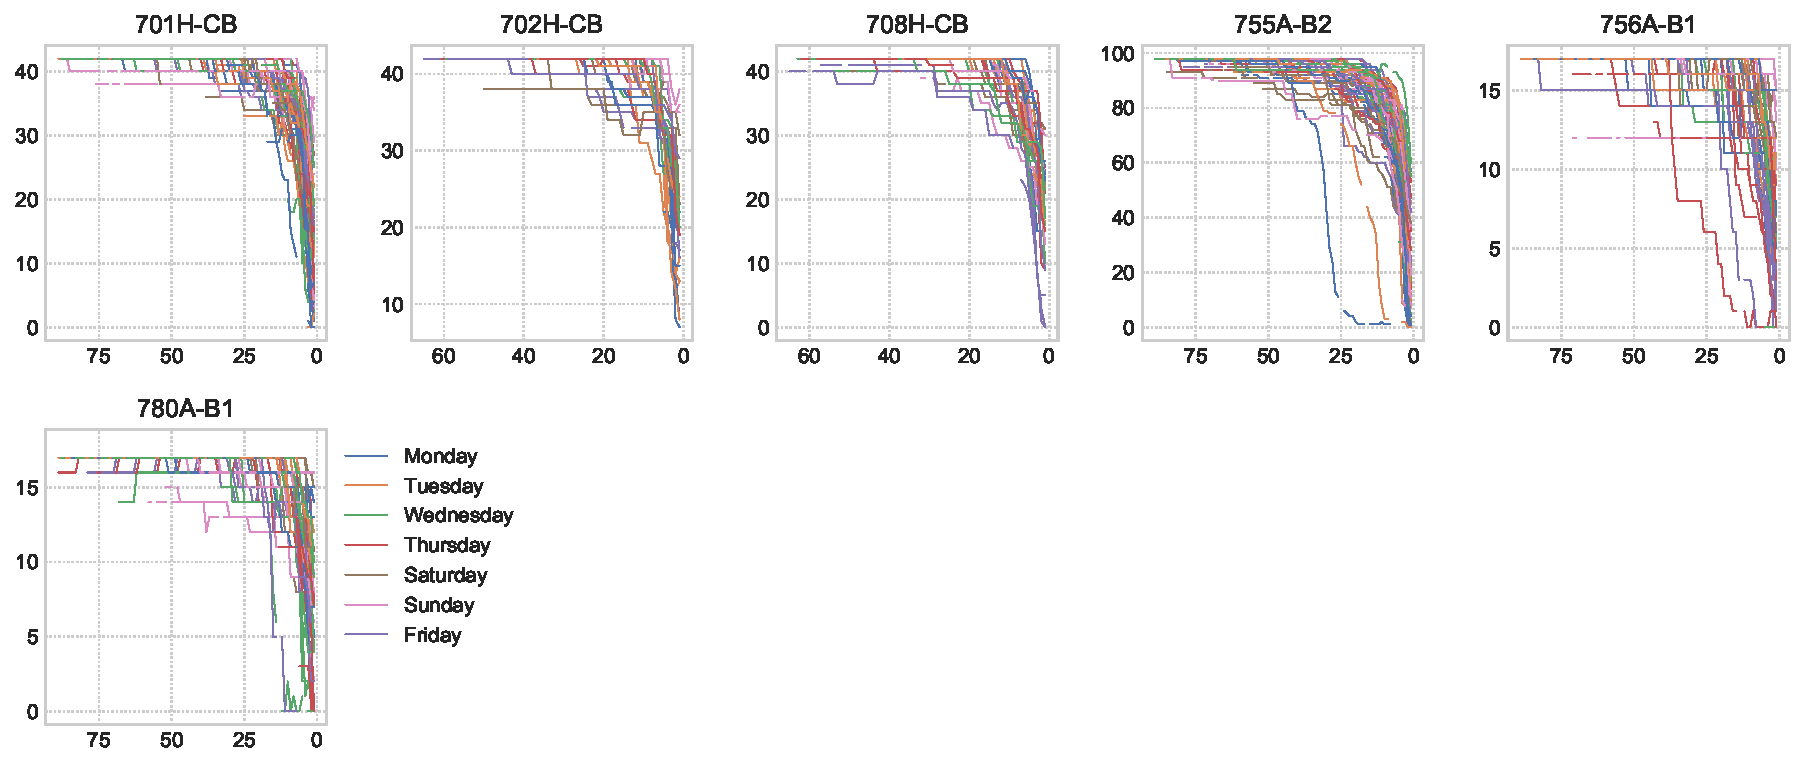
\includegraphics[height=0.92\textheight]{../data/figures/poorly_explained.pdf}
    \end{figure}

\end{frame}


\begin{frame}
    \frametitle{Главные компоненты}

    \begin{figure}
        \centering
        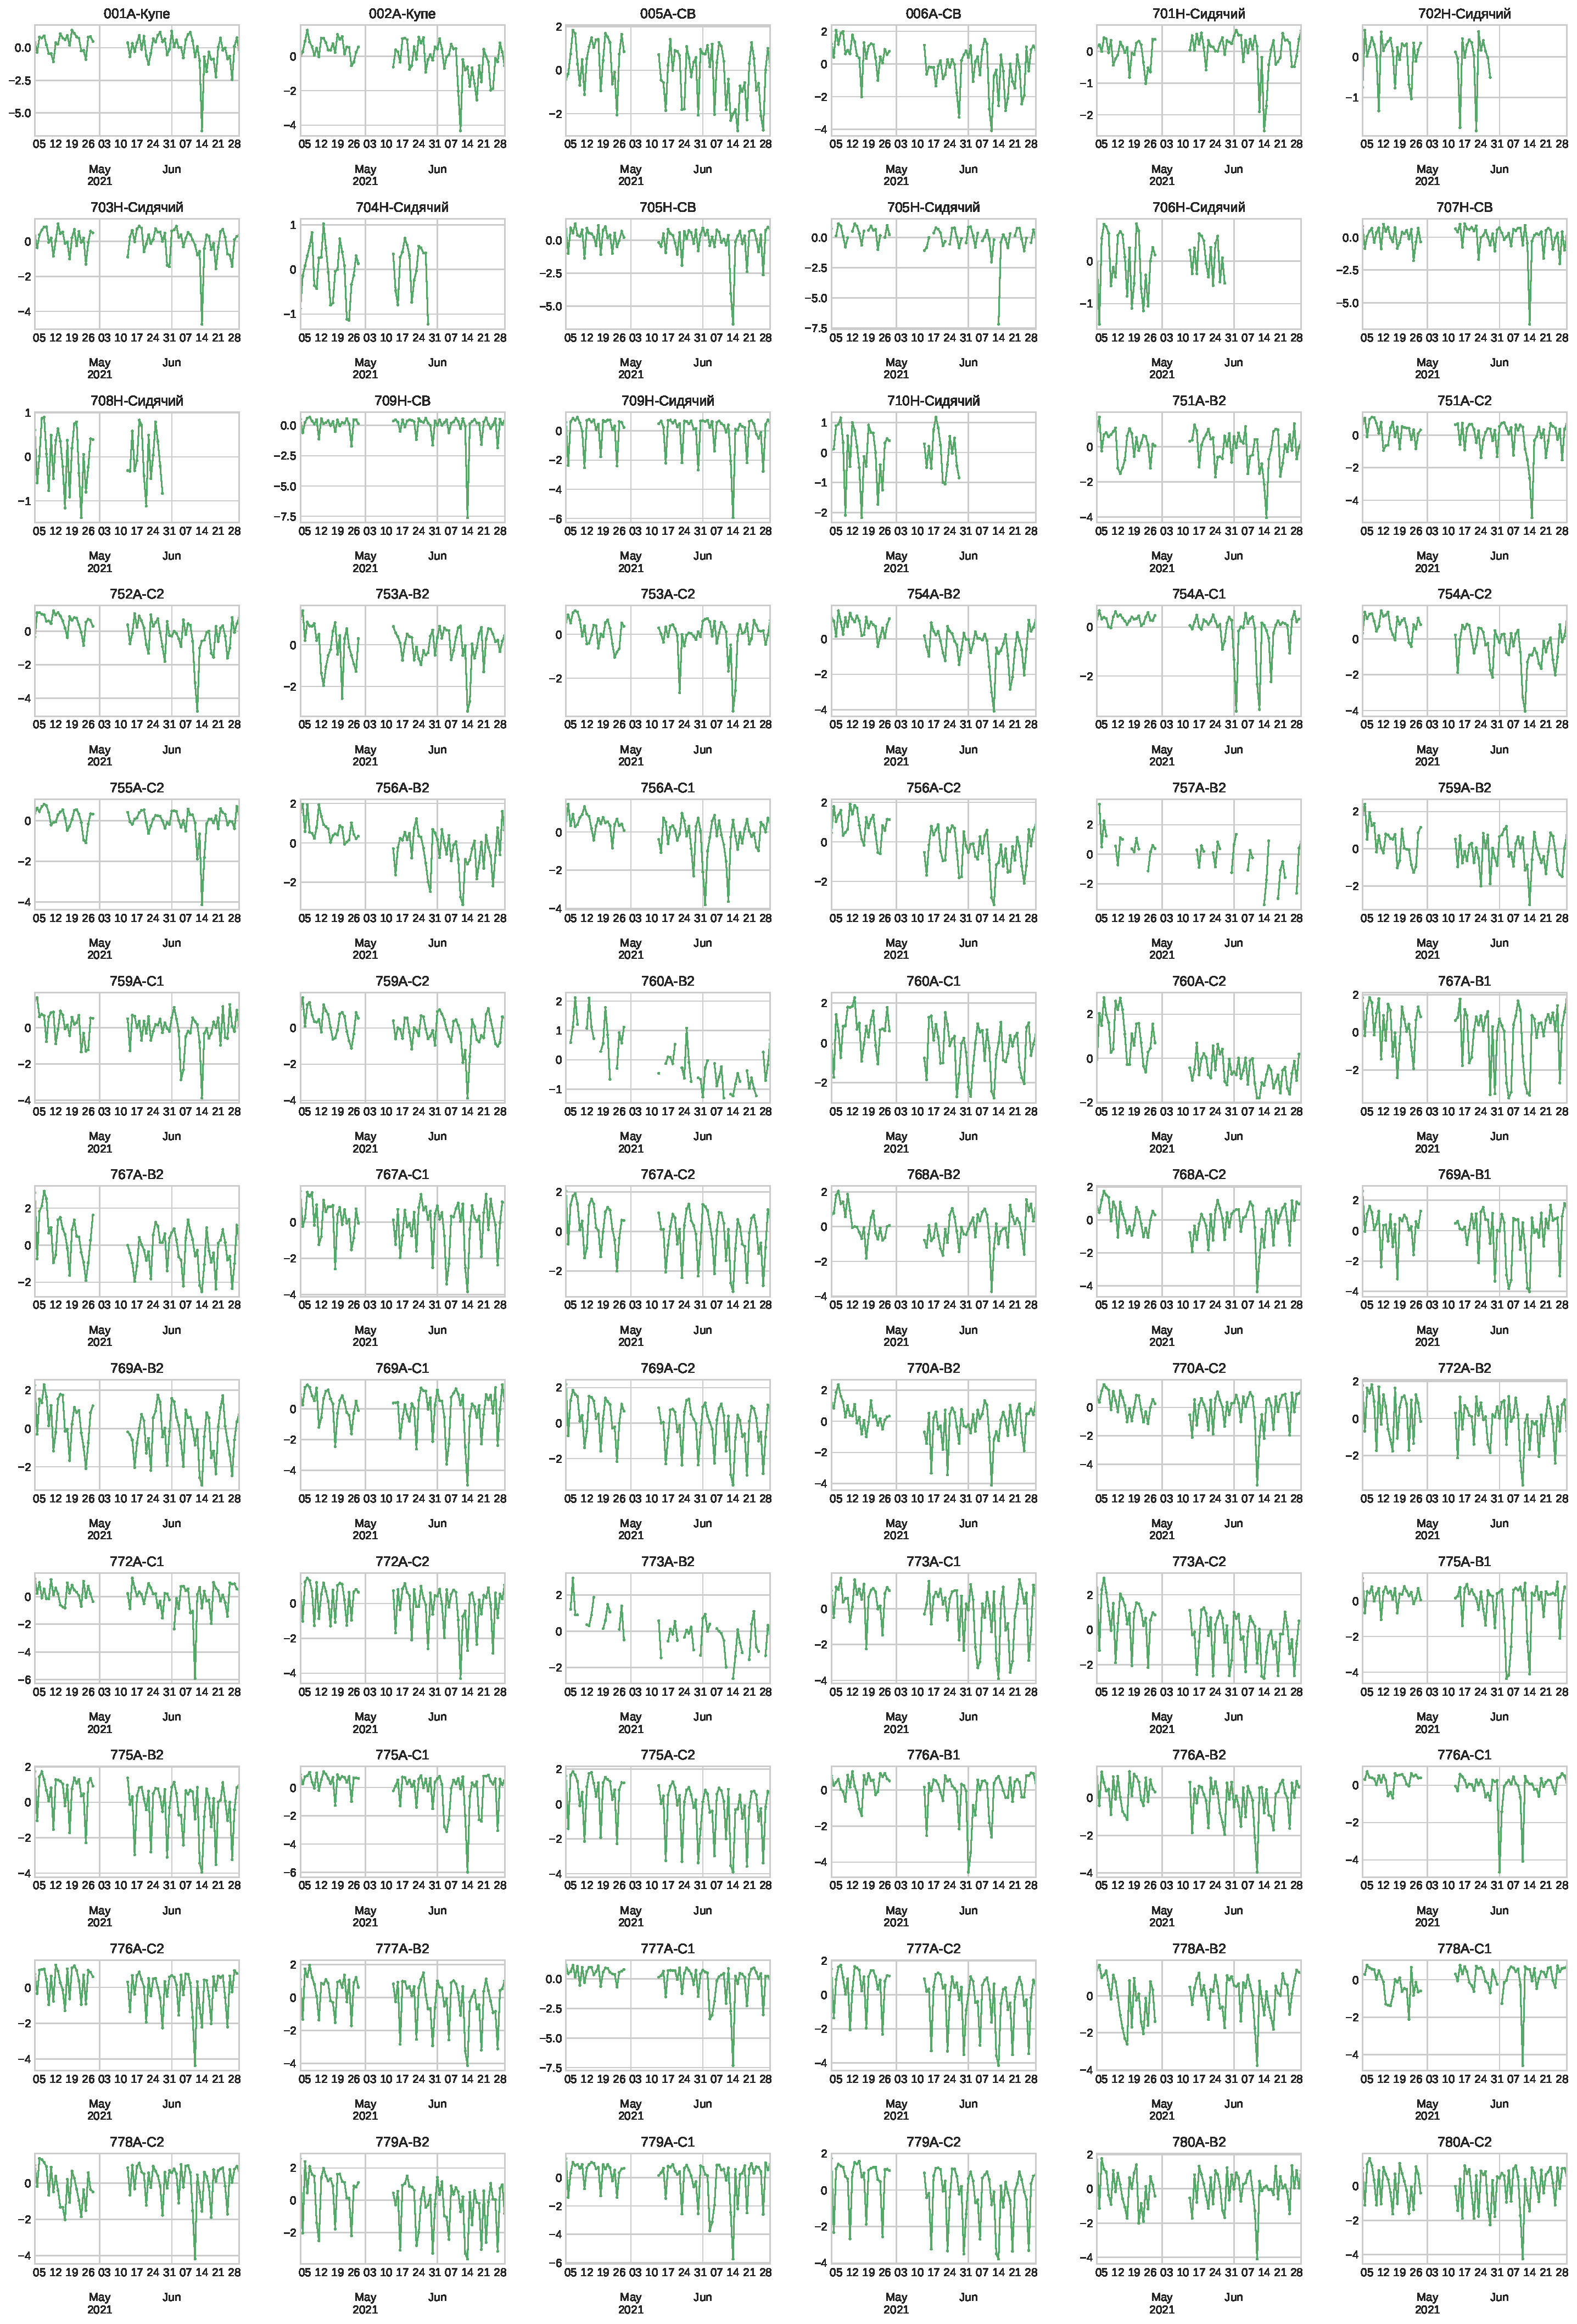
\includegraphics[height=0.92\textheight]{../data/figures/pcs.pdf}
    \end{figure}

\end{frame}


\begin{frame}
    \frametitle{Автокорреляции главных компонент}

    \begin{figure}
        \centering
        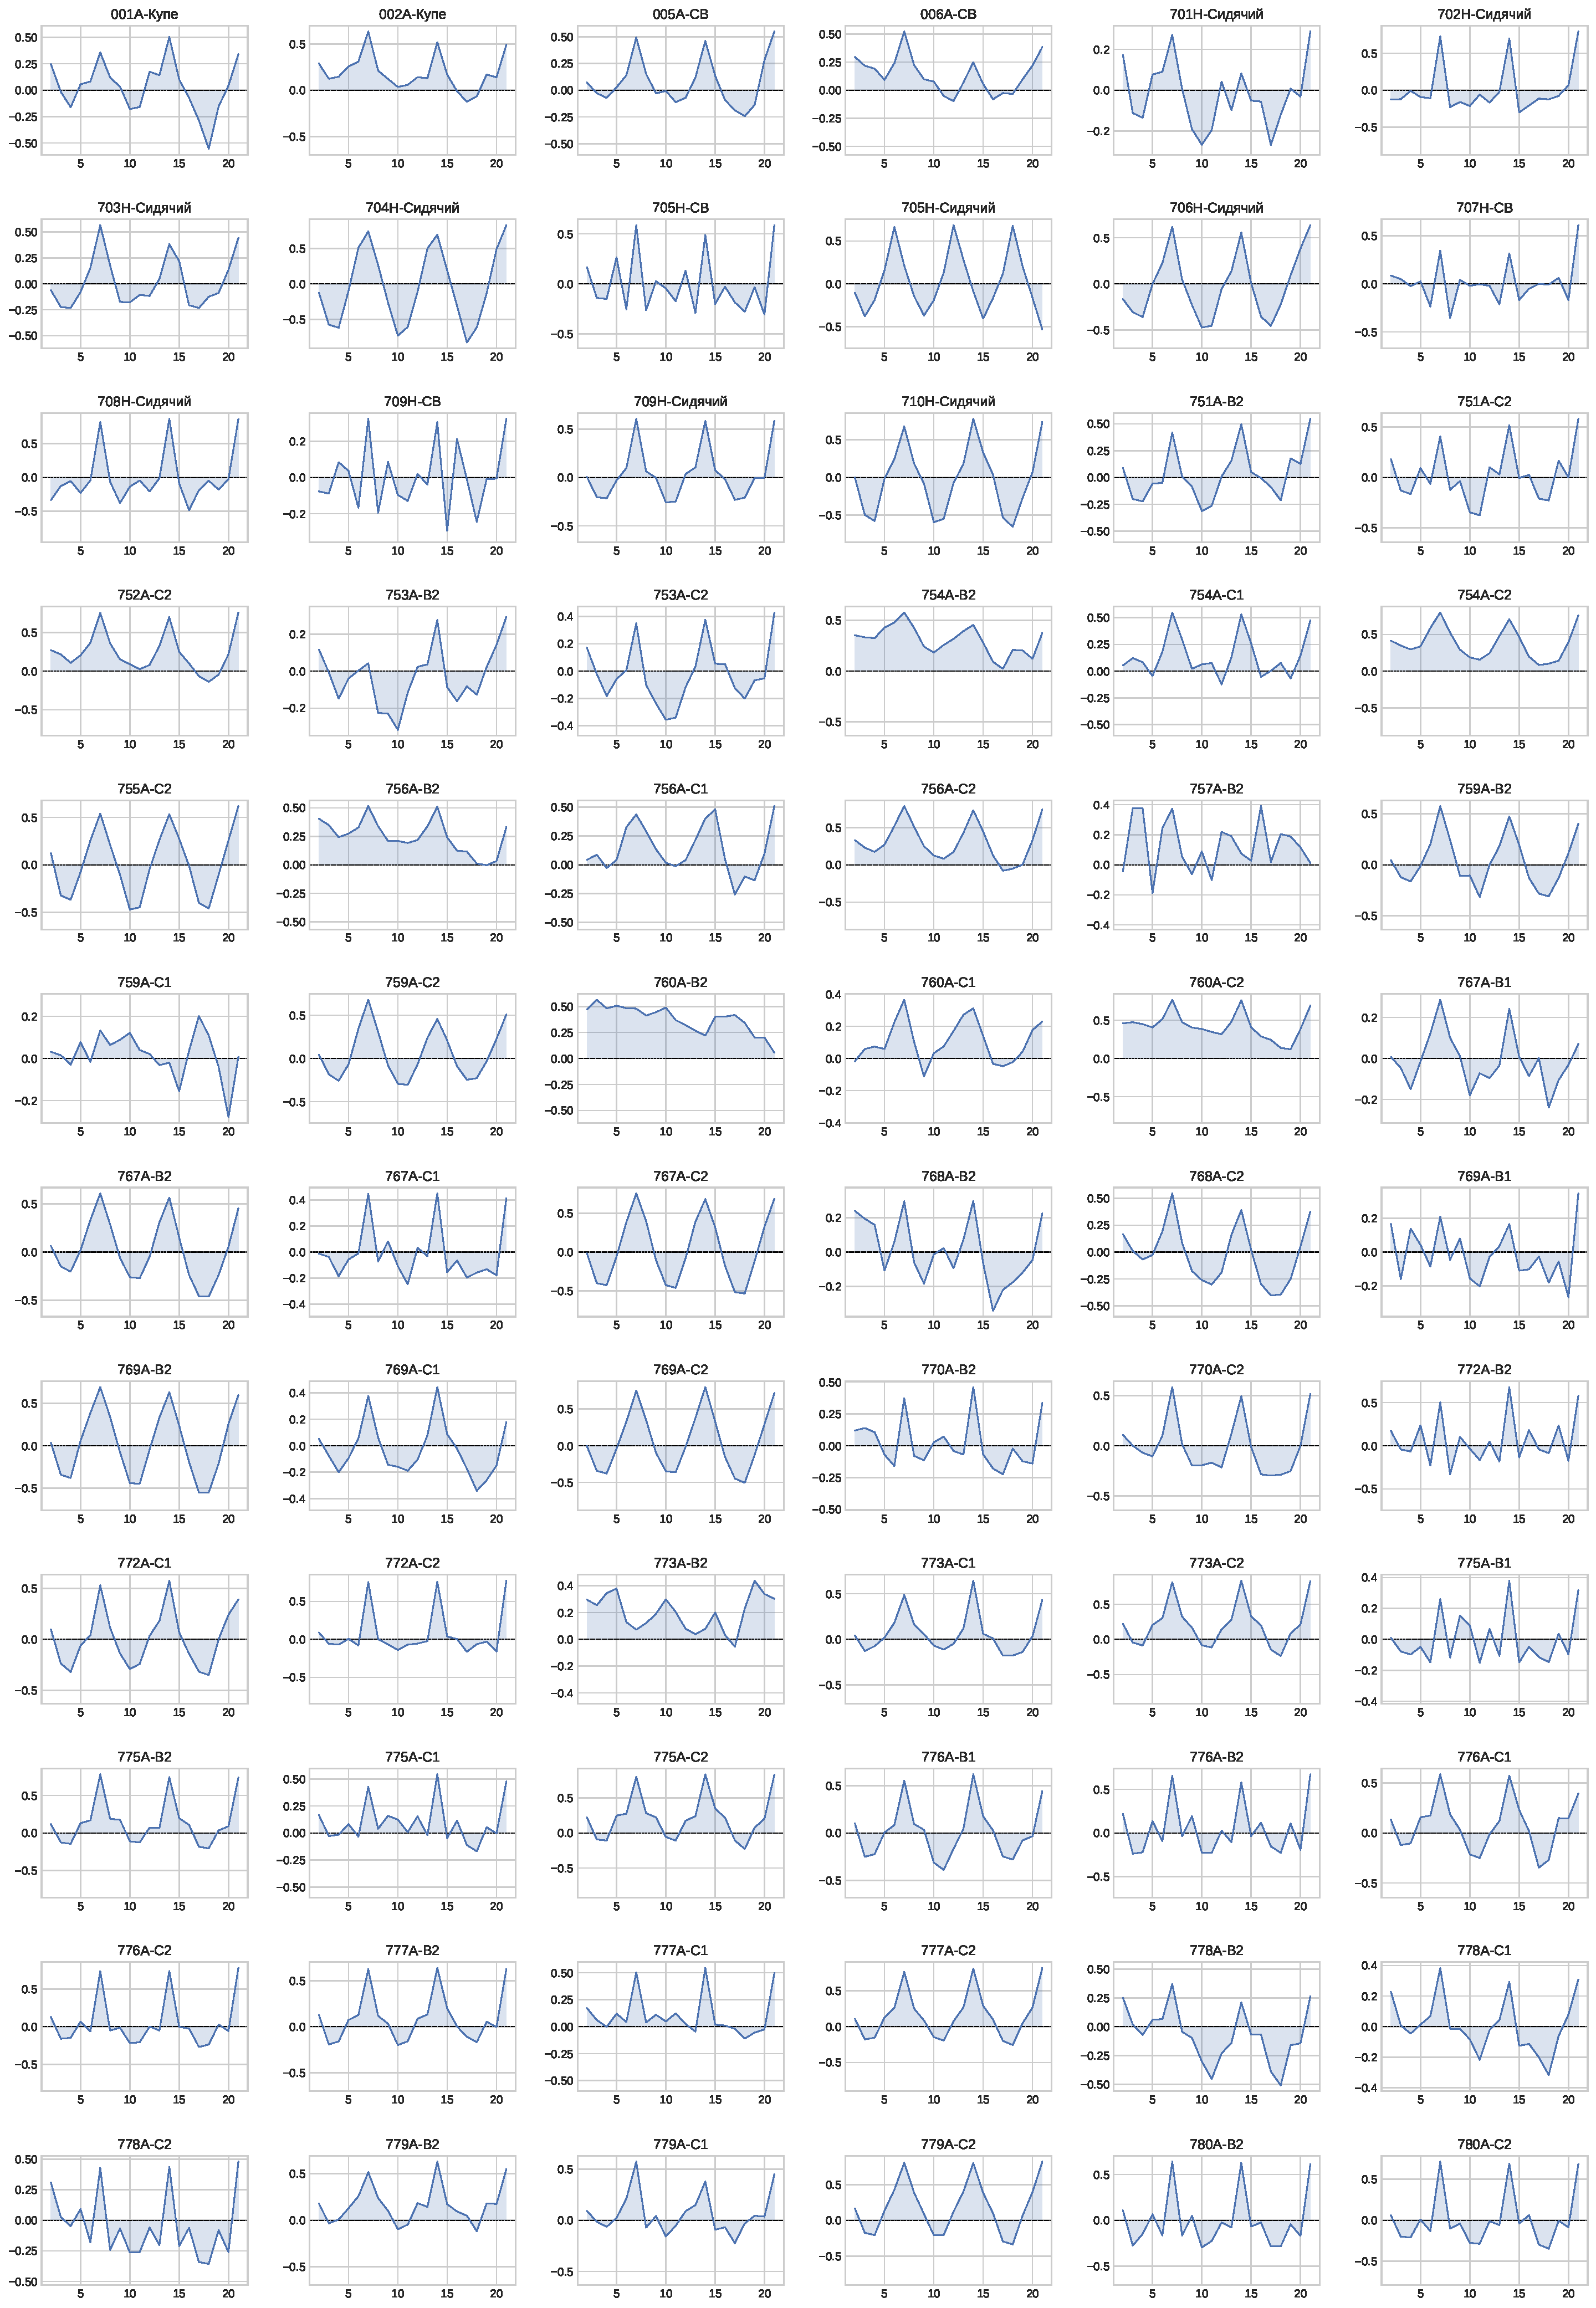
\includegraphics[height=0.92\textheight]{../data/figures/pcs_acf.pdf}
    \end{figure}

\end{frame}


\begin{frame}
    \frametitle{$\mu(\tau)$}

    \begin{figure}
        \centering
        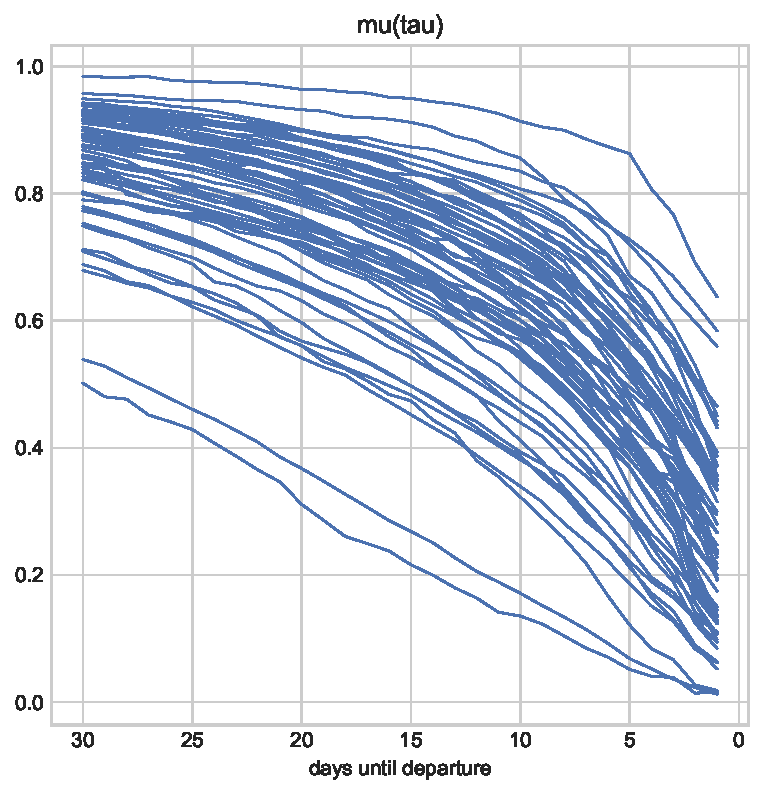
\includegraphics[width=0.9\textwidth]{../data/figures/means.pdf}
    \end{figure}

\end{frame}

\begin{frame}
    \frametitle{Кластеры $\mu(\tau)$}

    \begin{figure}
        \centering
        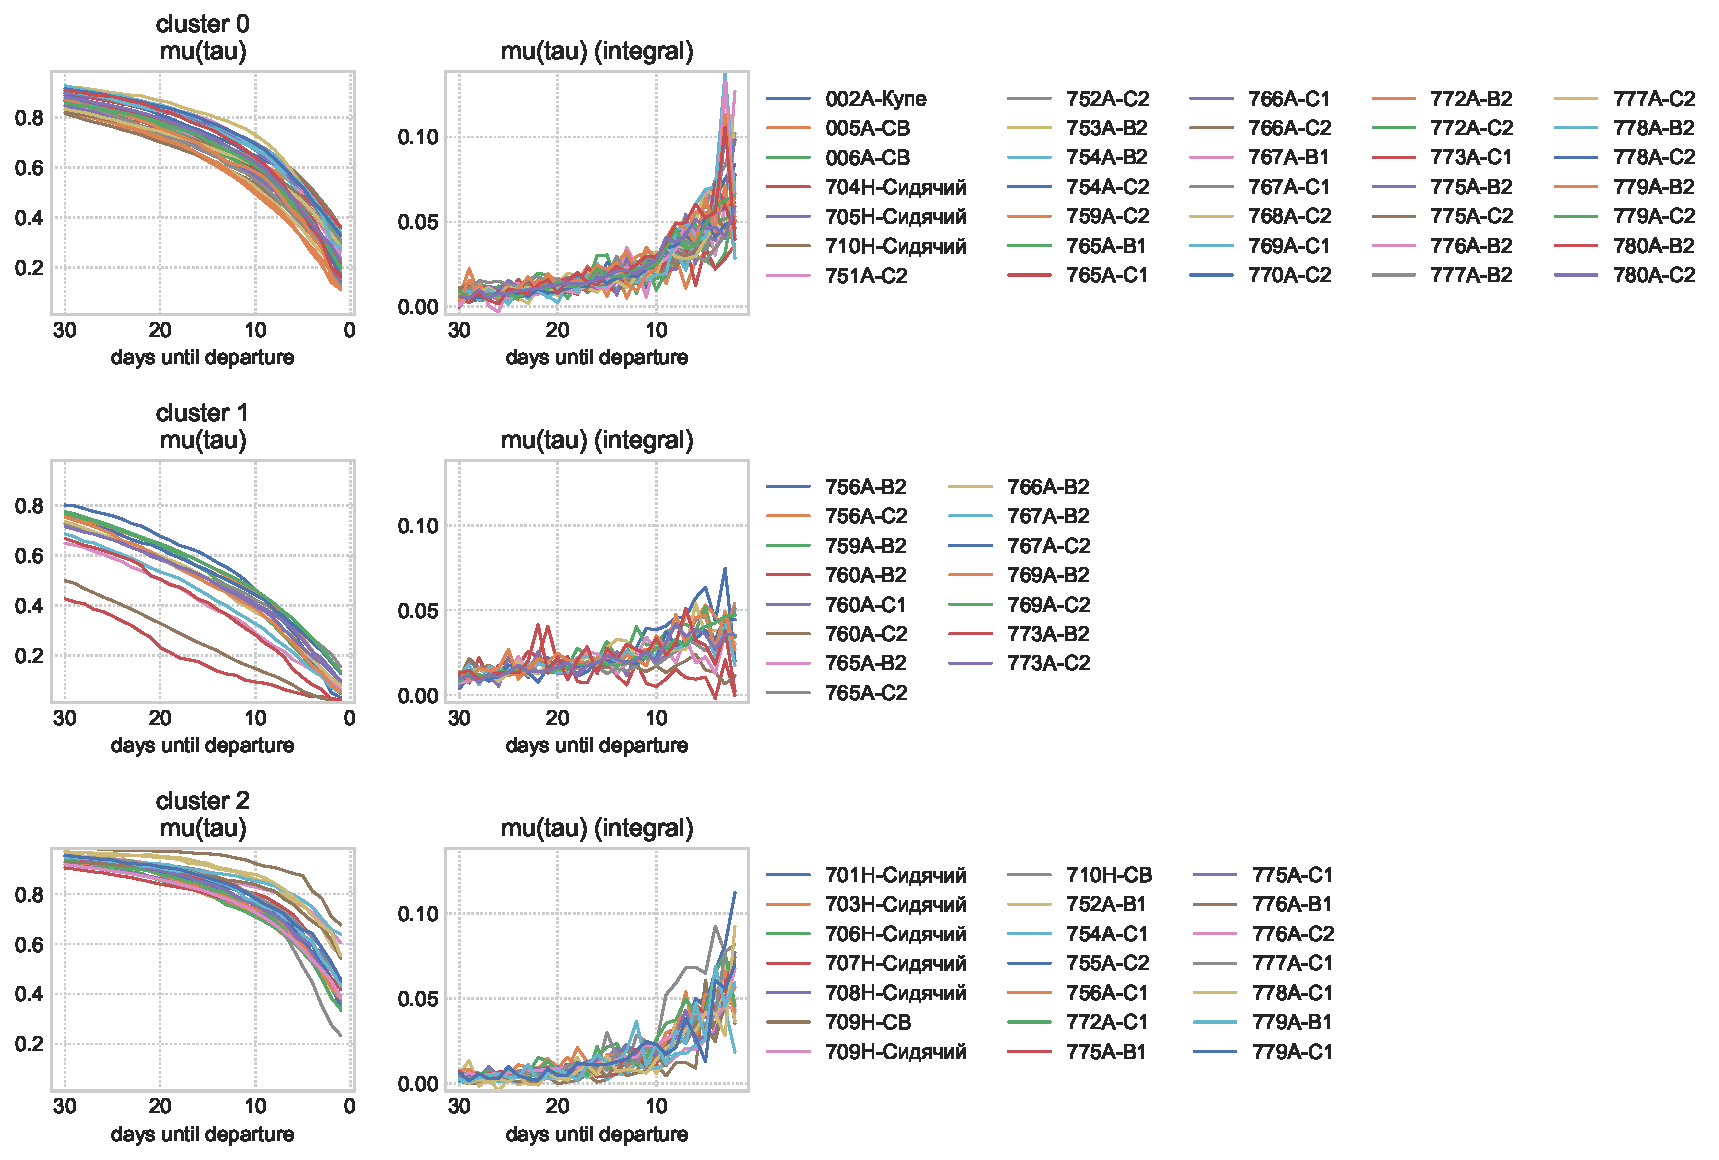
\includegraphics[height=0.92\textheight]{../data/figures/mean_clusters.pdf}
    \end{figure}

\end{frame}


\begin{frame}
    \frametitle{Объясняем кластеры $\mu(\tau)$}

    \begin{figure}
        \centering
        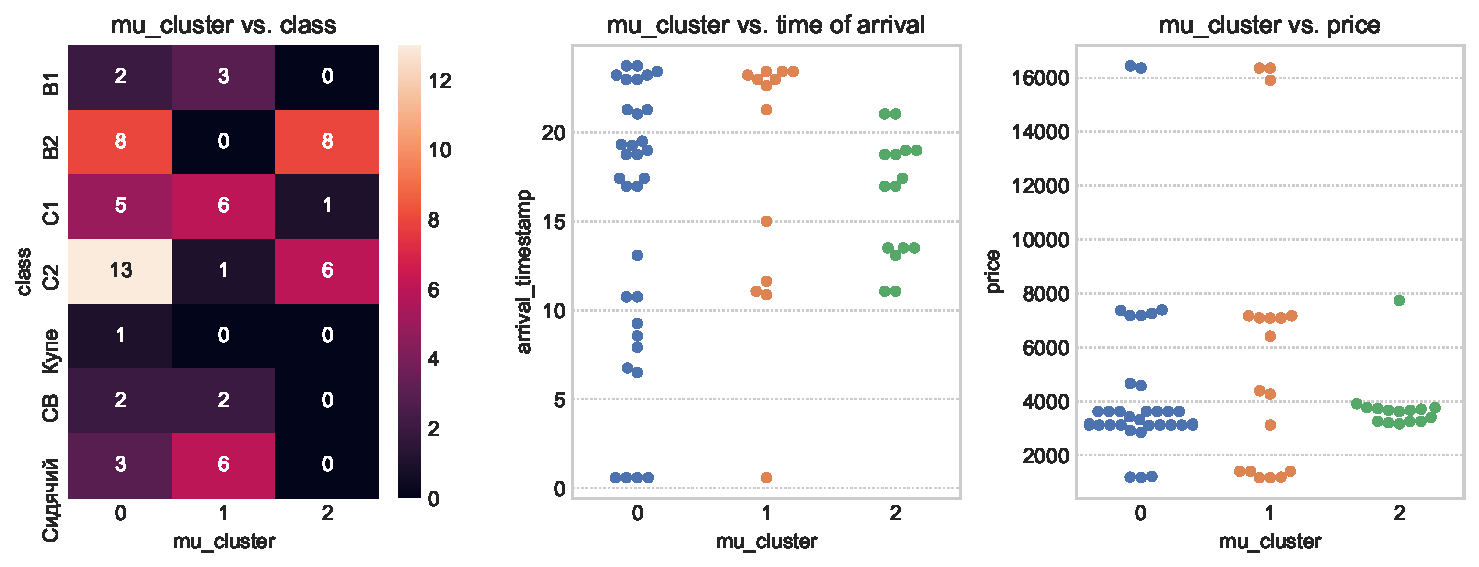
\includegraphics[width=\textwidth]{../data/figures/explaining_mean_clusters.pdf}
    \end{figure}

\end{frame}


\begin{frame}
    \frametitle{$V(\tau)$}

    \begin{figure}
        \centering
        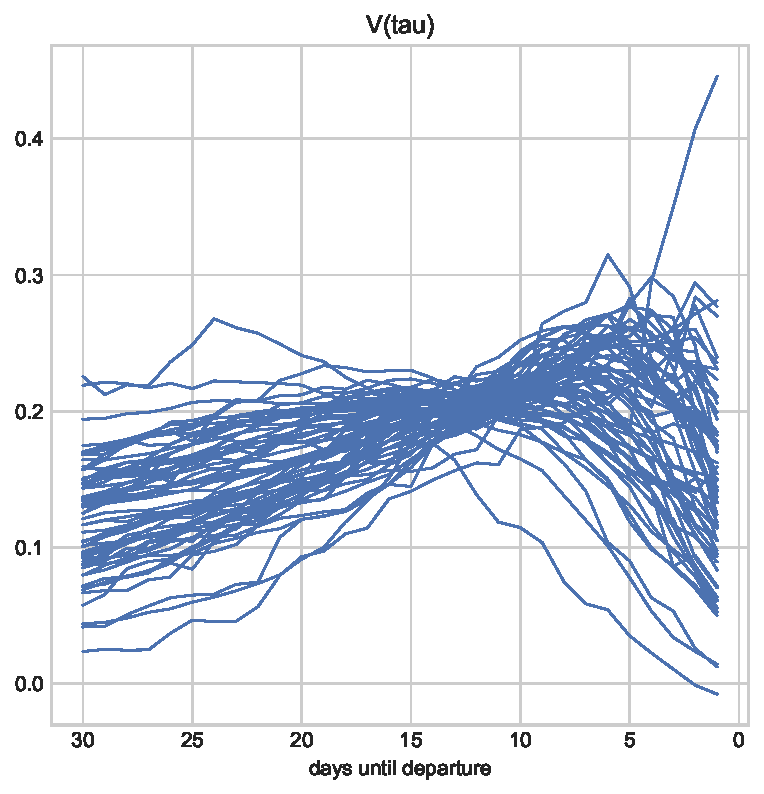
\includegraphics[width=0.9\textwidth]{../data/figures/eigenvectors.pdf}
    \end{figure}

\end{frame}

\begin{frame}
    \frametitle{Кластеры $V(\tau)$}

    \begin{figure}
        \centering
        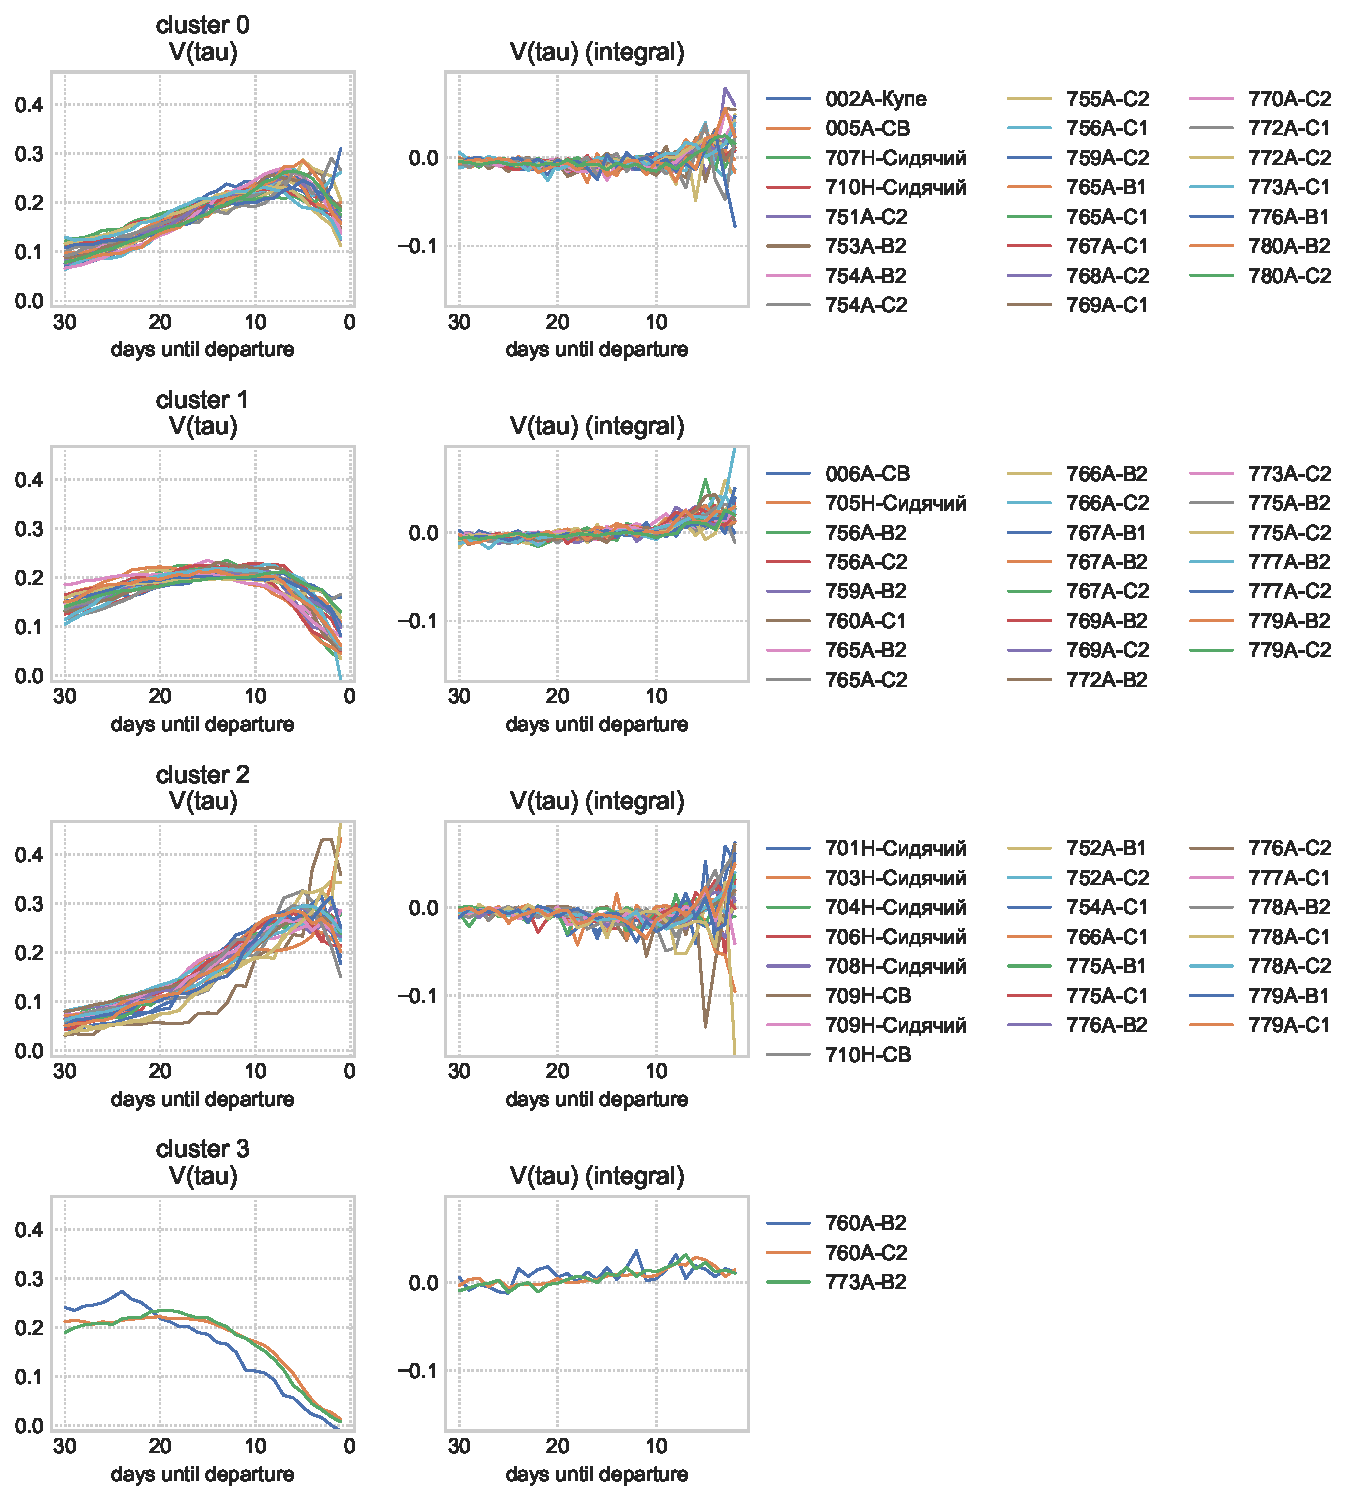
\includegraphics[height=0.92\textheight]{../data/figures/eigenvector_clusters.pdf}
    \end{figure}

\end{frame}


\begin{frame}
    \frametitle{Объясняем кластеры $V(\tau)$}

    \begin{figure}
        \centering
        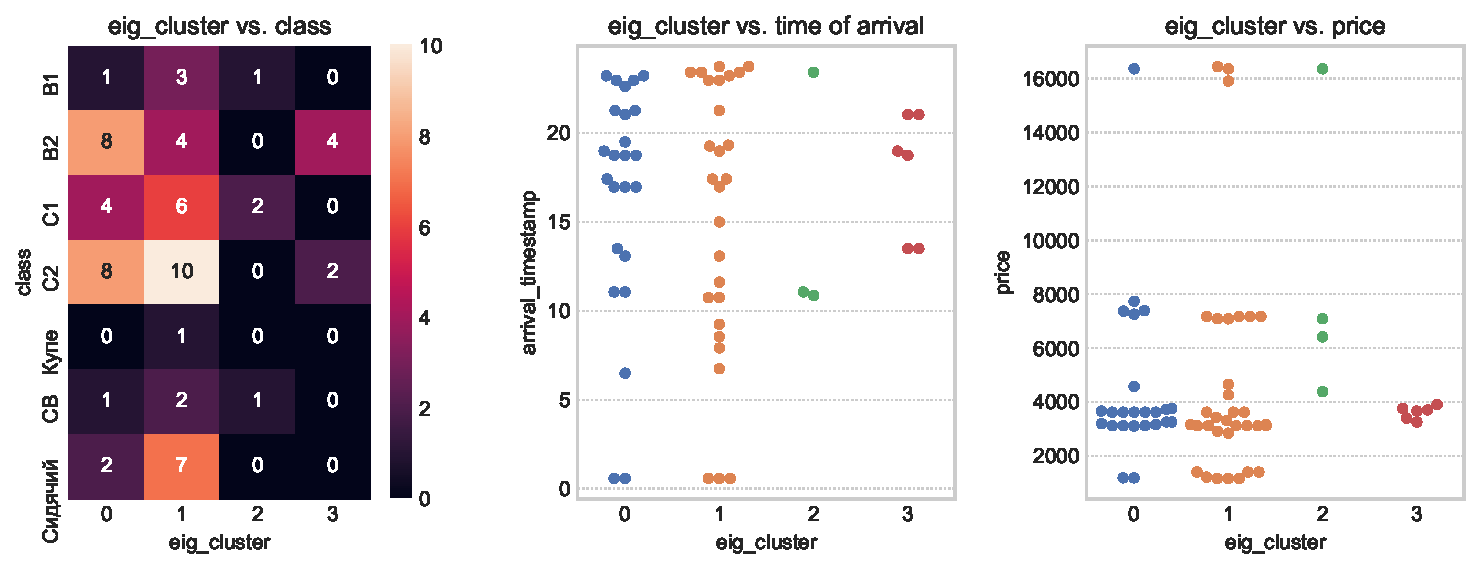
\includegraphics[width=\textwidth]{../data/figures/explaining_eigenvector_clusters.pdf}
    \end{figure}

\end{frame}


\begin{frame}
    \frametitle{Би-кластеры}

    \begin{figure}
        \centering
        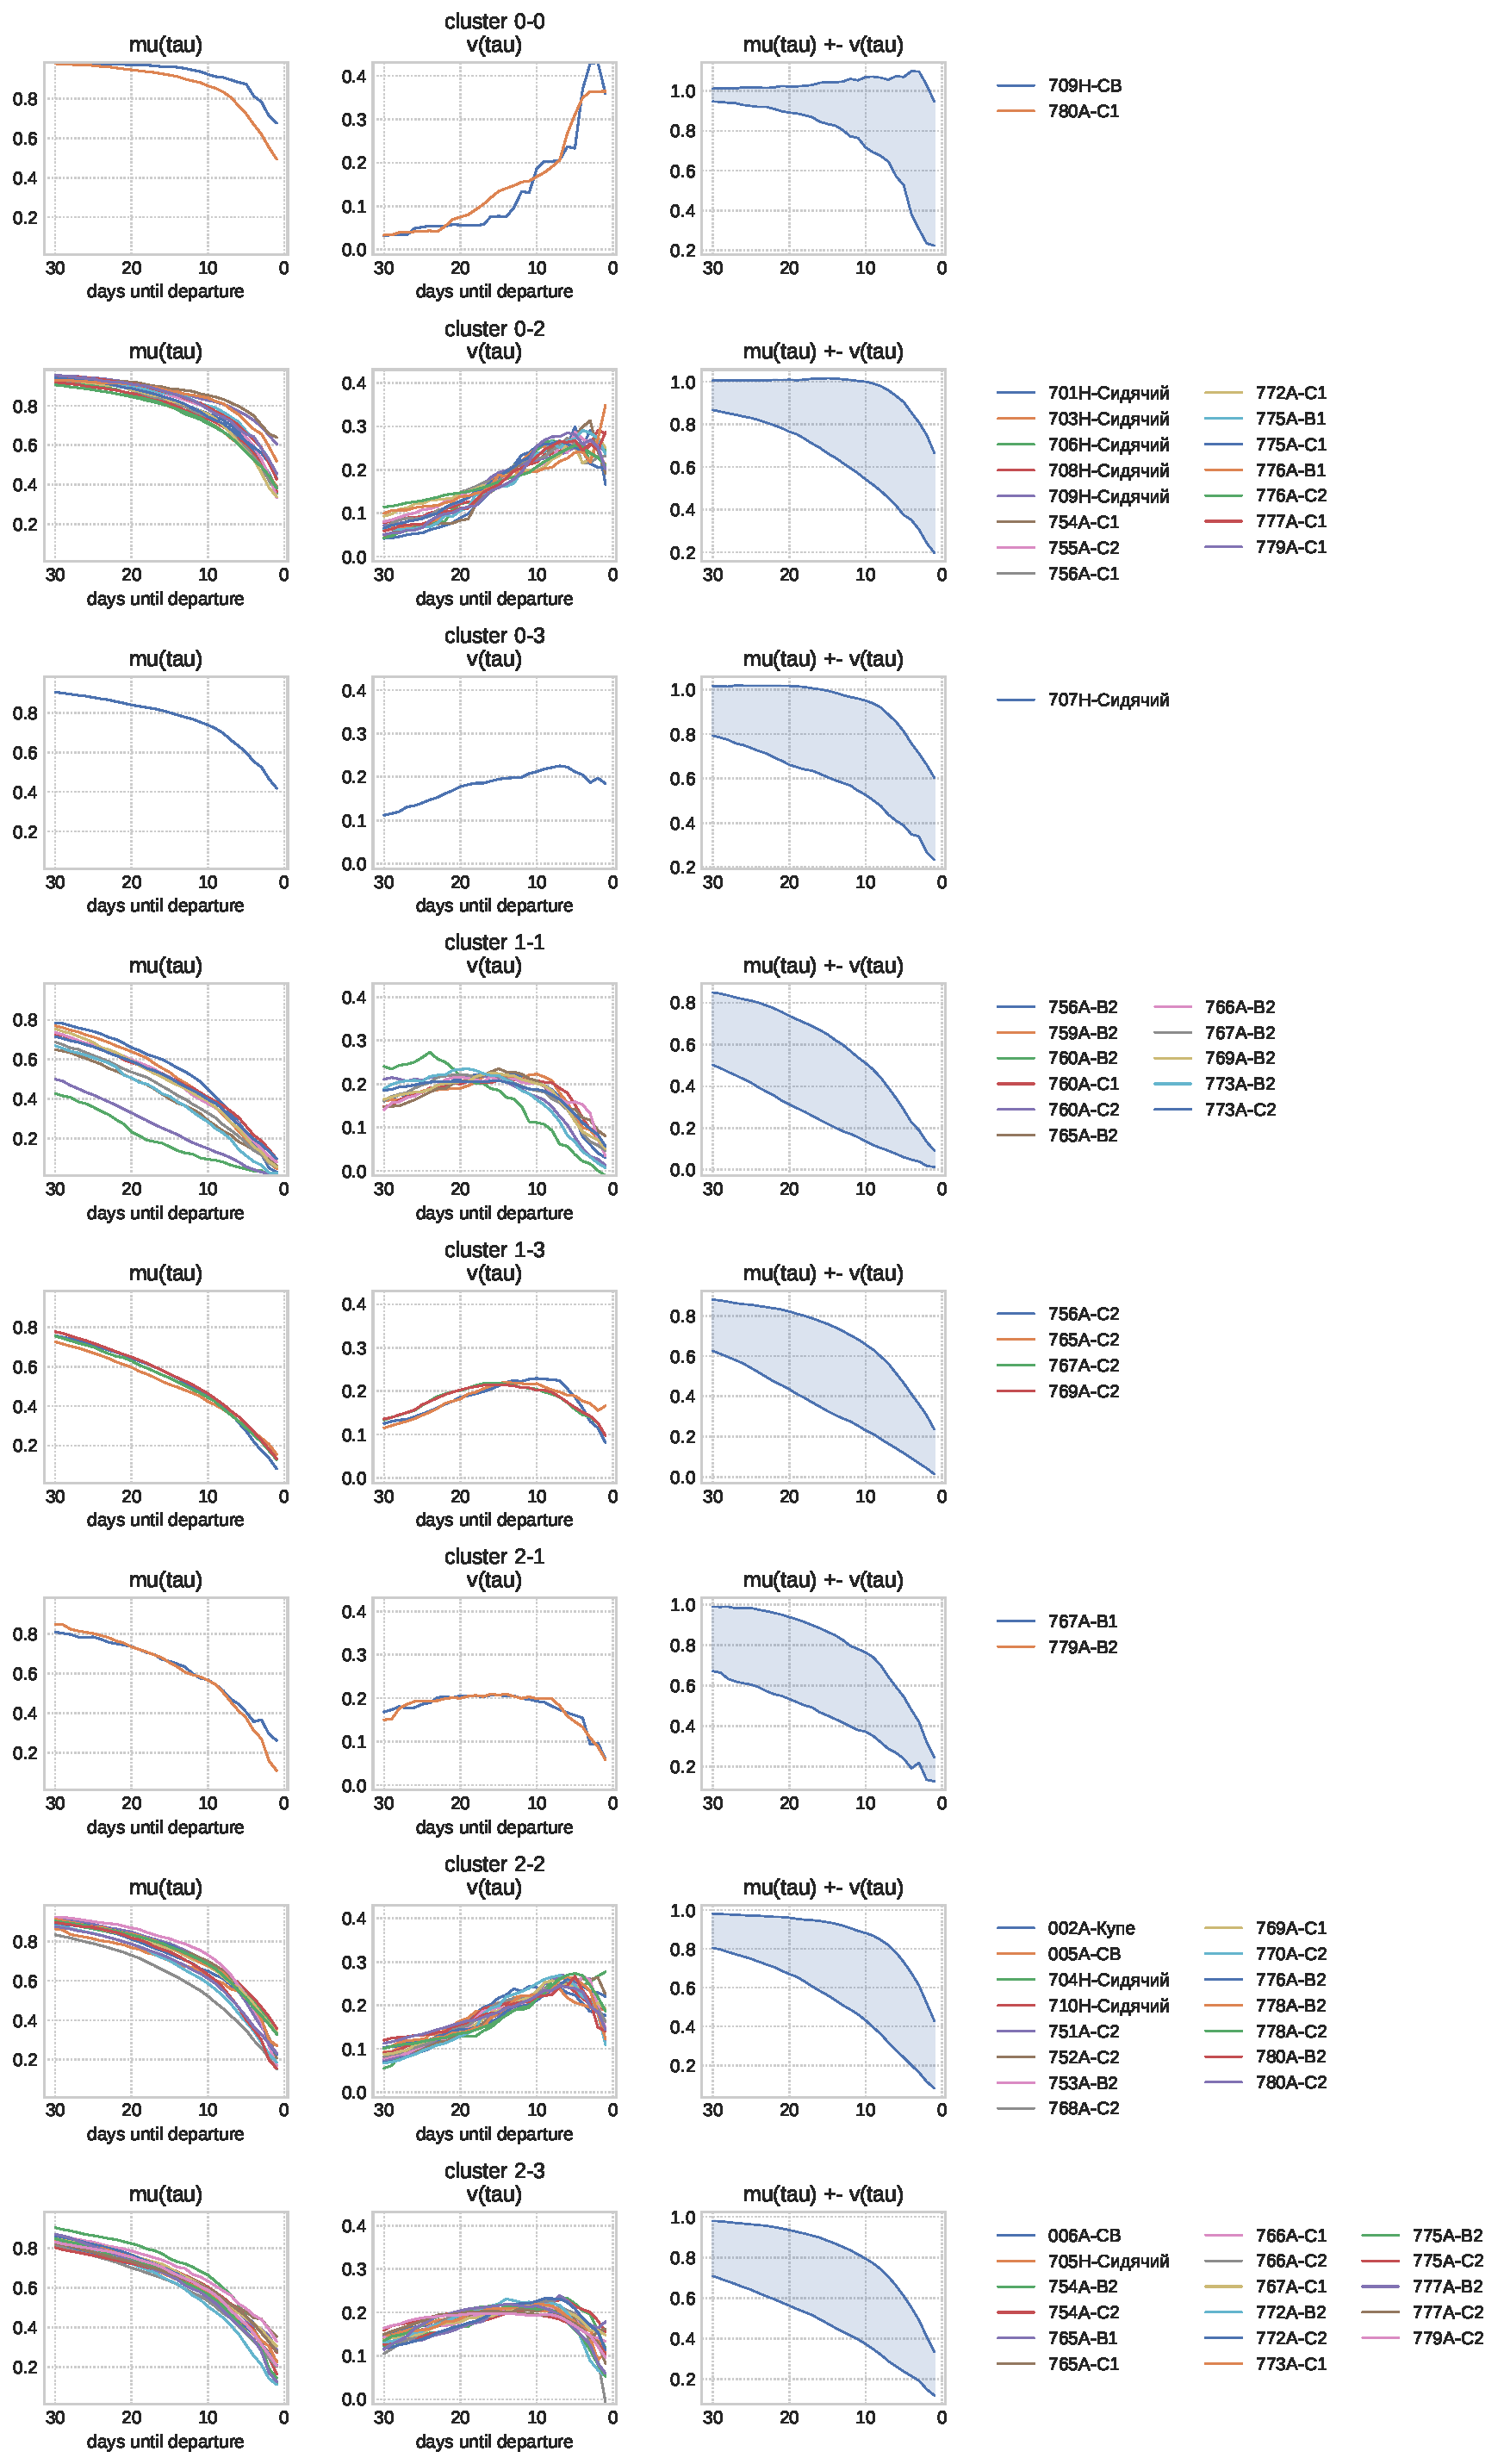
\includegraphics[height=0.92\textheight]{../data/figures/biclusters.pdf}
    \end{figure}

\end{frame}

\begin{frame}
    \frametitle{Объясняем би-кластеры}

    \begin{figure}
        \centering
        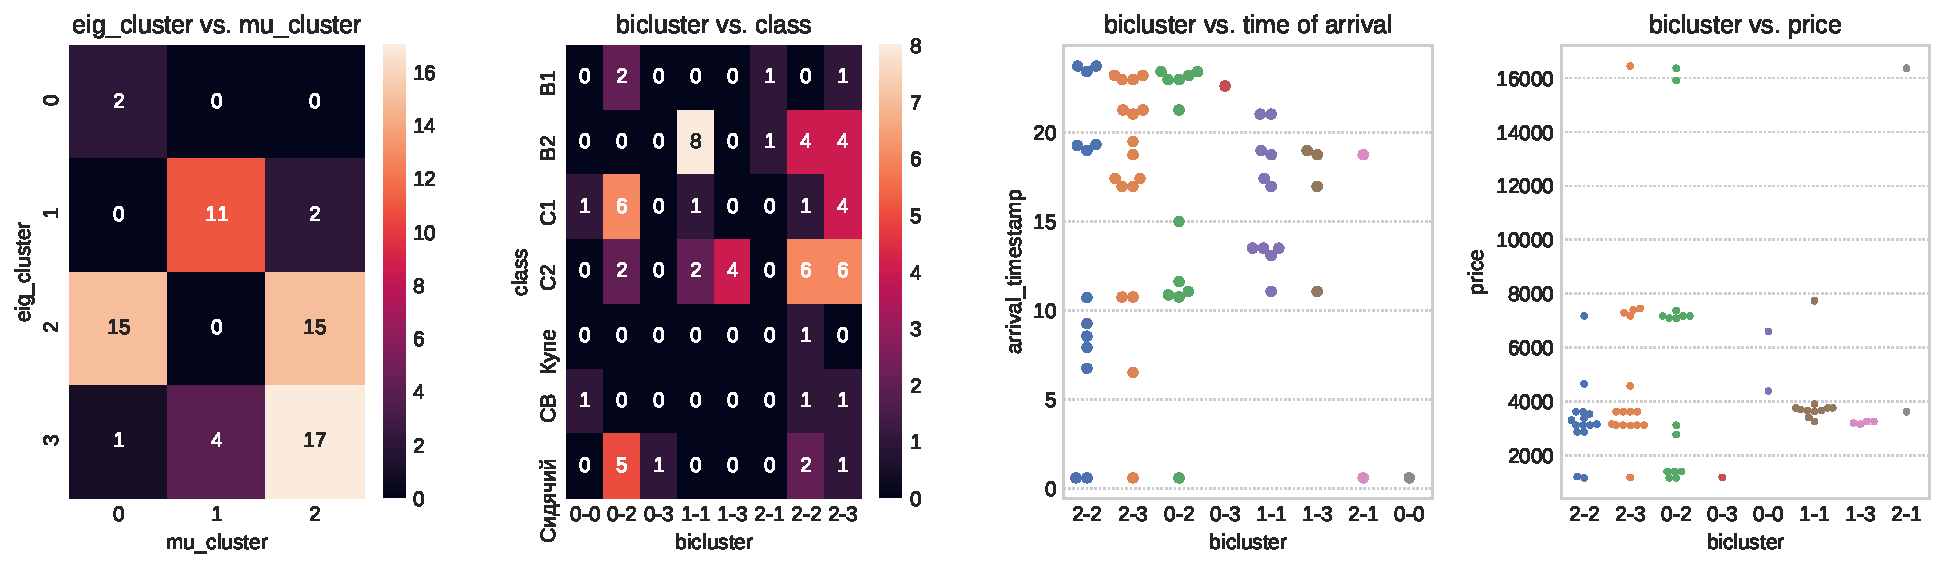
\includegraphics[width=\textwidth]{../data/figures/explaining_biclusters.pdf}
    \end{figure}

\end{frame}


\end{document}
